\chapter{\label{chap:researchSetting}Research Setting}


\minitoc



ABSTRACT:
In this chapter I introduce the research setting in which the empirical studies of this dissertation are conducted: rugby union in contemporary China.  In the previous chapter, I outlined a novel theory of social bonding through joint action.  This theory embraces accumulating evidence to depict a brain in the business of minimising ``free energy'' in the social environment. To do so, the brain relies on resources distributed throughout multiple layers of environment.  Within this paradigm, not only are other brains, bodies, and features of the immediate task environment important to shaping and constraining joint action.  In addition, the macro-context of cultural norms, conventions, and affordances also function to direct and finesse joint action in patterned and therefore predictable ways.  Anthropology—--a discipline with a proud history of attention to the details of cultural and ecological context, and now with a diverse methodological toolkit—--is well positioned to offer empirical evidence for a novel theory of social bonding through joint action.

Rugby union in contemporary China contains various layers of context that require explanation.  Together, the standardised parameters (rules, regulations, conventions) of rugby union, the psychological and cultural patterns typically existing in mainland China, and the specific history of modern sport and rugby union in mainland China collectively shape observable behaviour.  In the sections below, I introduce these three main contextual layers of the research setting, and conclude by updating theoretical predictions in light of the informational affordances likely to be present in joint action scenarios.  In addition, I explain the (unique) combination of qualifications that enabled me to conduct research in this specific context.




                                          \begin{CJK}{UTF8}{gbsn}

\section{The Temple of the God of Agriculture Sports Institute}
I first visited the Beijing Temple of the God of Agriculture Sports Technology Institute (\textit{Beijingshi xiannongtan tiyujishu yundong xuexiao} 北京市先农坛体育技术运动学校,
hereafter the Institute) first thing in the morning on my first Monday in Beijing.  I entered via the main entrance in the south and made my way west to the main administration building by hugging the southwest perimeter of the 30,000 seat capacity, multi-purpose sport stadium that spatially dominates the Institute's campus (see map ~\ref{fig:beijingXNT}). My aim that morning was to confirm the details of my proposed research with the vice principal of the Institute responsible for the rugby program, as well as the head coach of the rugby program.  I knew both the vice principal and the head coach from previous times spent in China studying (2006 and 2008) and coaching and coaching rugby (2013) prior to my doctoral research, and although I had already received positive responses from both during the planning stages of my research, I still needed to confirm arrangements for research face-to-face.

I received mixed reactions when I announced to friends within the Chinese rugby community in Beijing that I was preparing to conduct research with the Beijing rugby team at the Institute. Those who were well reasonably well acquainted with the politics involved in rugby in China, Beijing, and sport in China more generally, warned me about becoming too involved,  perhaps because they were worried that I might suffer a similar fate to the group of coaches and athletes involved in the National Games in 2013.  Chinese rugby elder Adrian, for example (see Chapter ~\ref{chap:intro} Section ~\ref{sect:adrian}), warned me to be careful, citing that the Institute was riddled with ghosts: ``There really are ghosts there, I'm telling you Lijie, you should keep your distance'' (真的有鬼啊,我告诉你李杰,你最好离远点吧).  I naturally scoffed at these warnings, which were admittedly tongue-in-cheek. I was intrigued, however, to learn more about the cultural, political, and psychological---as well as ancient cosmological---principles that lay beneath the history of the Institute.

The Institute is located in the heart of Beijing, just to the west of Yongding gate in on the South 2nd Ring Road. As one can imagine given Beijing's 3000-year history, the centrally located land on which the Institute sits was not always home to sport facilities and professional athletes.  The Institute takes its name from the temple that was built on the land in during the Ming Dynasty in the 15th century.  Yongding gate marks the southern end of the city's ancient north-south axis, which also includes, from south to north: Tiananmen Square, the Forbidden City, Jingshan Park, and the Drum and Bell Towers (see Figure ~\ref{fig:beijingTemplesXNT}).  For thousands of years, Chinese cities have been laid out on a north-south axis according to the principles of feng shui. The auspicious power or energy (\textit{qi} 气) of each monument along this axis is believed to flow upward from the south (south being the most auspicious and therefore important of the Four Directions in Chinese cosmology).

In addition to this spatial dimension, dynastic powers also sought to reinforce the cosmological order temporally, through regular performances of a system of Grand, Middle, and Common Sacrifices.  In the Ming and Qing Dynasties, Emperors (or their commissioned representatives) used the Temple of the God of Agriculture (hereafter the Temple of Agriculture) during the middle month of Autumn and Spring (according to the Chinese lunar calendar), to perform Middle Sacrifices (in a system of Grand, Middle and Common Sacrifices) in honour of the Harvest (\textit{nong} 农)---one of the four main cosmological principles, in addition Heaven (\textit{tian} 天), Earth (\textit{di} 地), and Ancestors (\textit{zu} 祖)\citep[98]{Brownell2008}.  When the Qing Dynasty (1644---1912) finally buckled under the pressure of Western Imperial occupation and popular revolutionary political movements in 1912, however, Confucian Sacrifices in Beijing's various temples ceased.  But as one form of ritual expired in China, another form began.

The embrace of the practice and spectacle of modern sport by the Republic of China (ROC, 1912-1948) and the People's Republic of China (PRC, 1949-present) has been so resounding and fundamental that sport stadiums (and the sporting events for which these stadiums were specifically constructed) have supplanted ancient temples and rites along Beijing's sacred north-south axis as a medium of communicating state order \citep{Brownell1995}.  The flow of auspicious cosmological energy now begins with the Temple of Agriculture Sports Institute (founded in 1930) in the south, and ends 21km to the north where the National Stadium, National Aquatic Centre, and the Olympic Green---the iconic monuments of the Beijing 2008 Summer Olympics---are situated.  Since re-joining the International Olympic Committee in 1979, China's athletes have participated at every Summer and Winter Olympics (except for the 1980 Moscow Summer Olympics, which China joined 65 other nations in boycotting following the Soviet Union's invasion of Afghanistan in 1979), winning over 600 medals in 28 different sports.  China's elite performance on the international stage is facilitated by a now enormous state-sponsored competitive sport system (\textit{jingji tiyu tizhi} 竞技体育体制), which consists of thousands of sport programs housed in secondary and tertiary level education institutions and specialist sport institutes throughout China's 34 provincial level regions.  According to China's National Bureau of Statistics, in 2016 China's sport industry reached a total scale of RMB 1.9 trillion yuan (USD300 billion).  Since 2014, when the central government first declared plans for sport to become a ``pillar industry'' of China's modern economy, the sport industry has been growing by an average of 18.2\% per year.  The central government has set a target total scale of 5 trillion yuan (USD800 billion) or 2\% of GDP by 2025.\footnote{For comparison, in 2016 the scale of the US sport industry was USD400 billion. At present, the Chinese sport industry is dominated by manufacturing (sport equipment, apparel, etc).  There is therefore considerable room in the Chinese sport sector for much higher value inputs, such as the development of the sports services (tournaments, leagues, activities).}

Sport first became associated with the Temple of the God of Agriculture, in the form of a horseracing track at the southern gate of the Temple at the end of the Qing dynasty. Beginning in this period of history, not all of the energy that has flowed from the sacred temple has been auspicious, however.  As I will explain below, the arrival of rugby to the Institute has been a predominant source of much of the most recent cosmological turbulence. Although I was personally captivated by the fact that the Institute was located in such a culturally meaningful location in Beijing, I was also slightly apprehensive about the state in which I was entering the Program and the Institute.  It was with a slight pang of nervousness, therefore, that I made my way from the southern gate, around the stadium, and towards the main office building to meet the Institute's vice-principal.


\begin{figure}[htbp]
  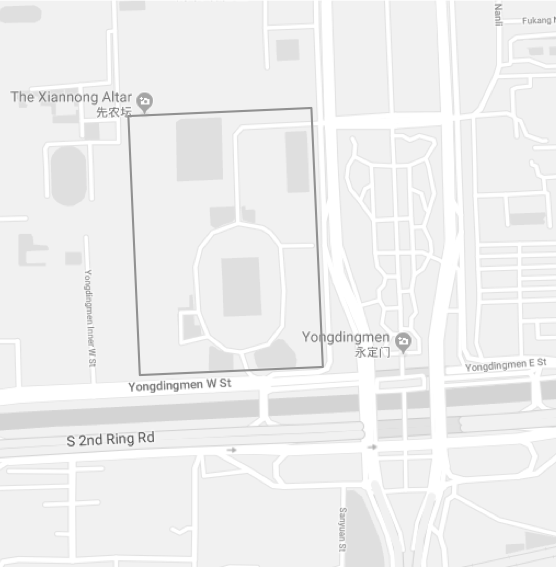
\includegraphics[width = \linewidth]{images/beijingXNT.png}
  \caption{Location of the Temple of the God of Agriculture Sports Technology Institute  (Source: Google Maps)}
  \label{fig:beijingXNT}
\end{figure}


\begin{figure}[htbp]
  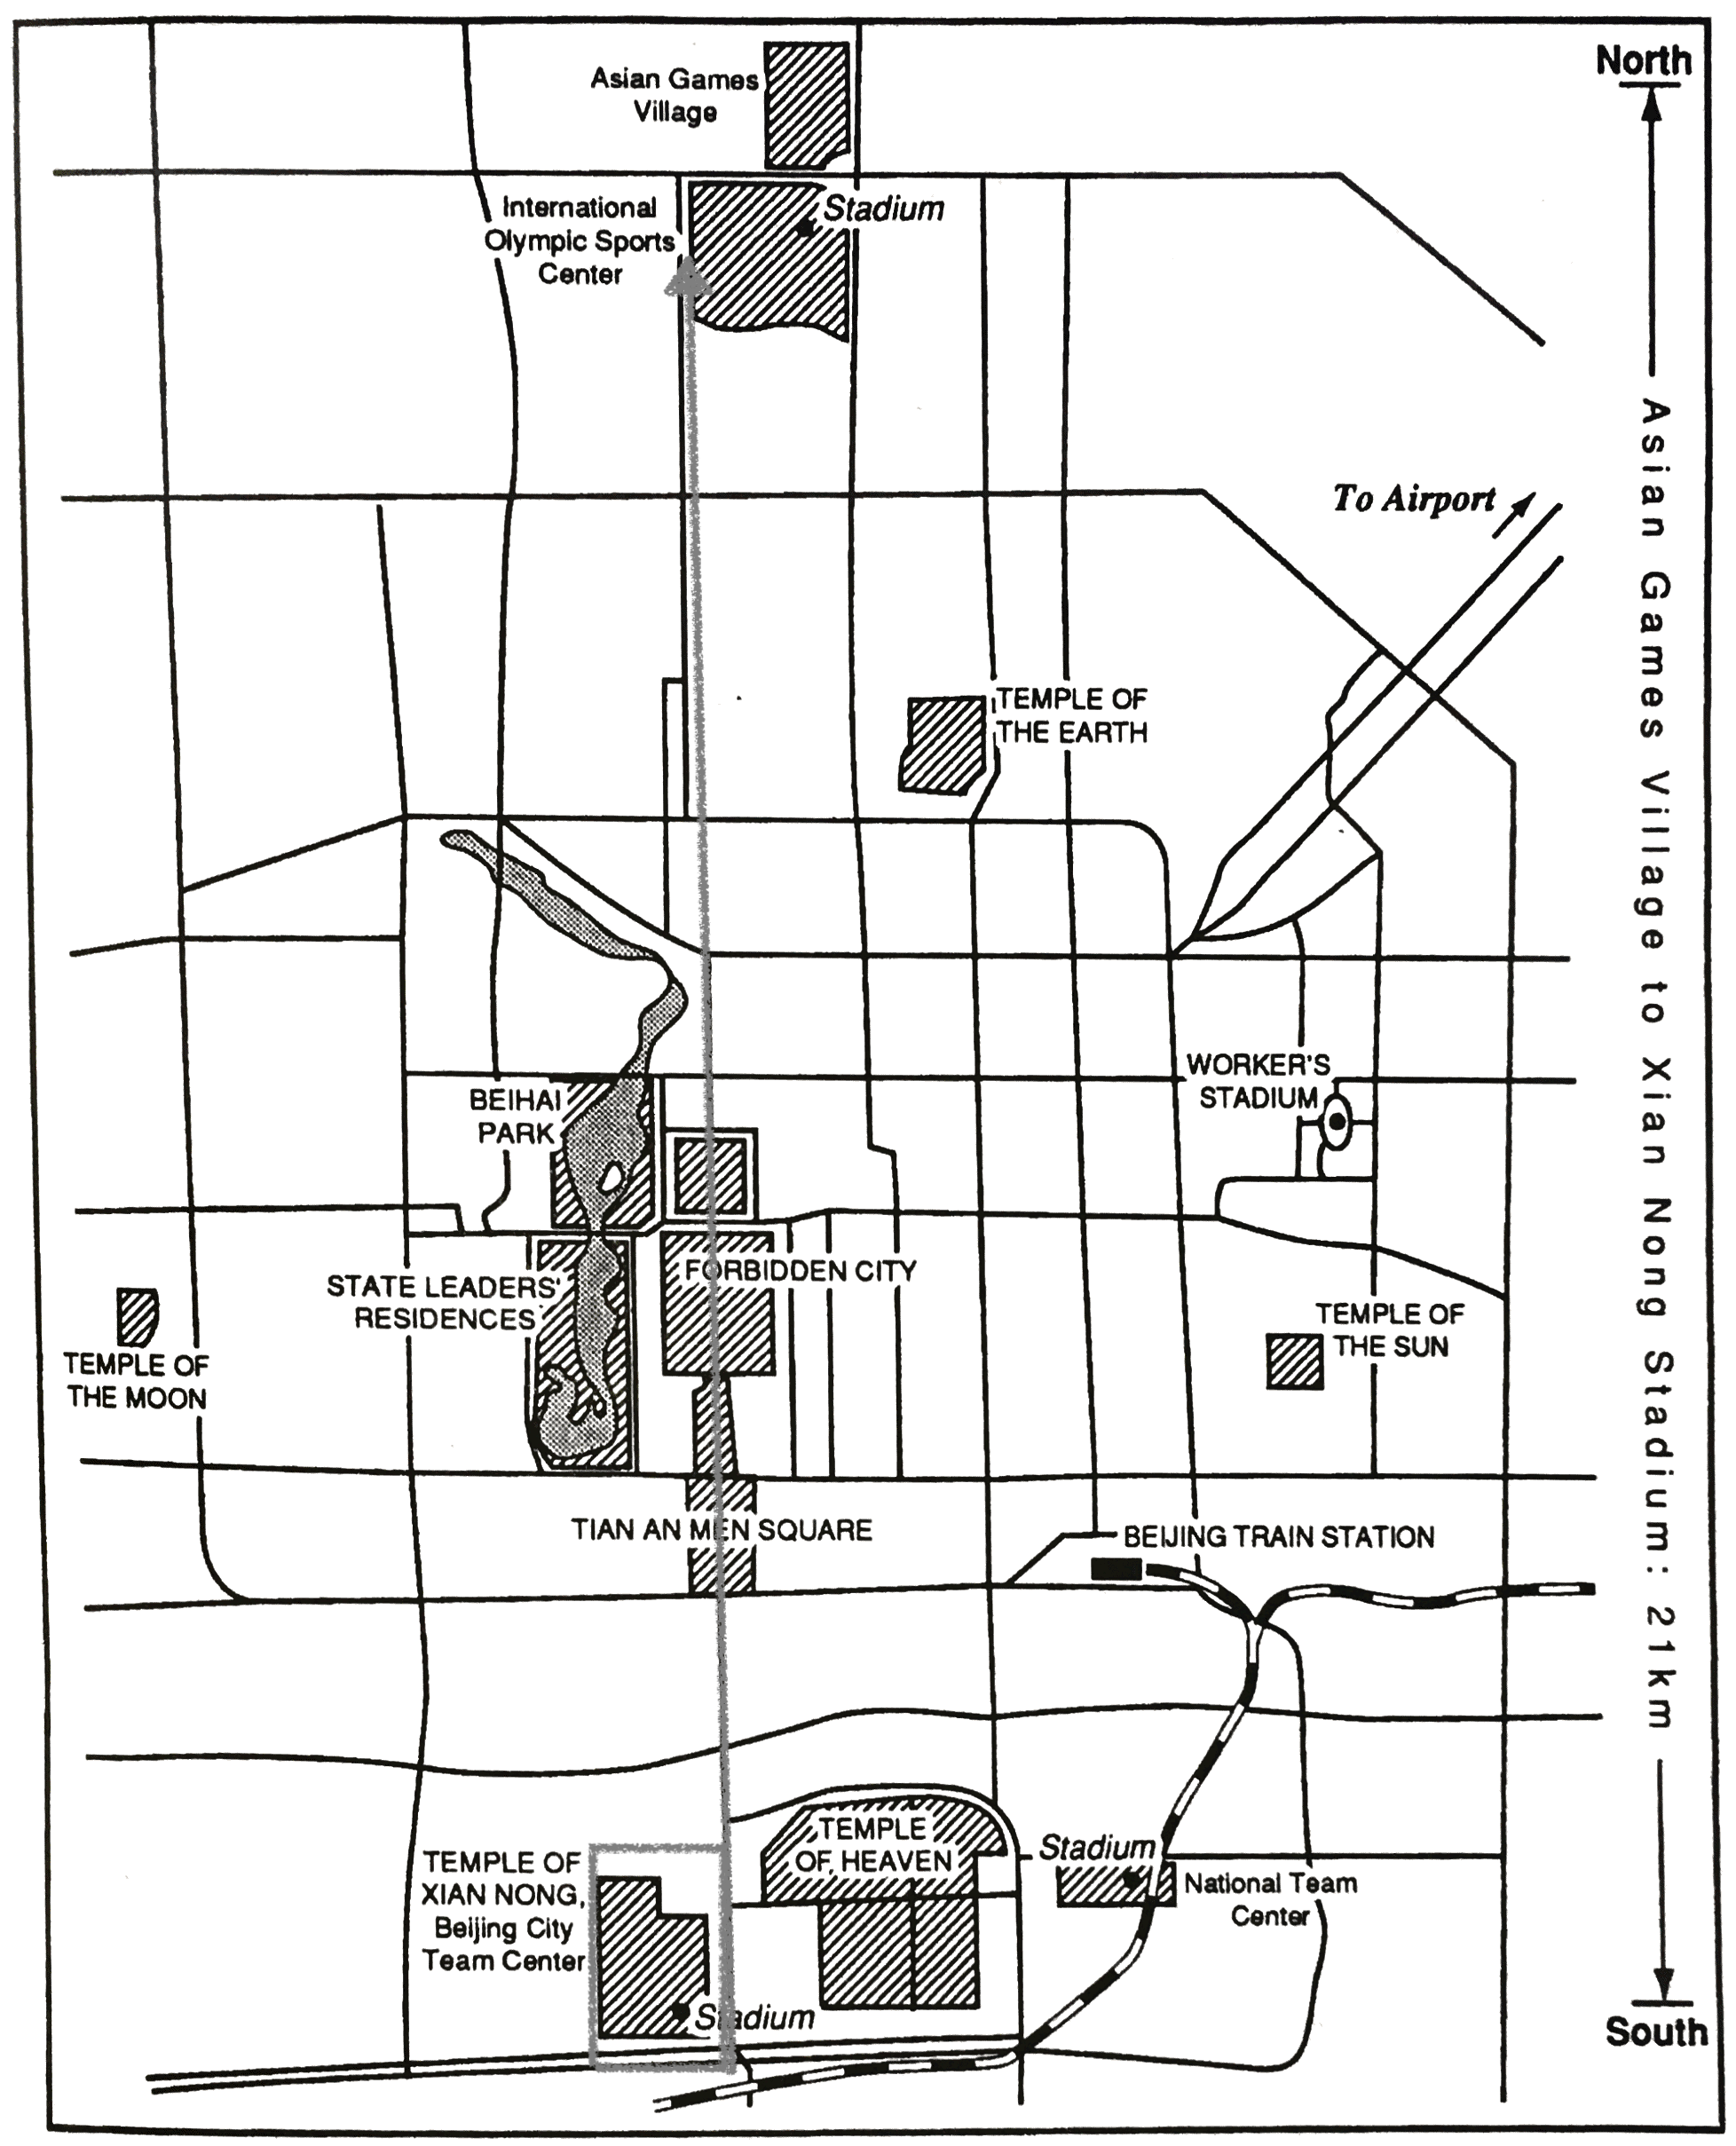
\includegraphics[width = \linewidth]{images/beijingTemplesXNT.png}
  \caption{Locations of former Qing dynasty temples (Brownell 2008)}
  \label{fig:beijingTemplesXNT}
\end{figure}




\section{Introducing the research setting}

Deciphering evidence for theories of human behaviour in real world settings presents a formidable challenge to science.  \textit{In situ}, human behaviour confronts the observer ``all at once''; often the precise causal mechanics operating to produce the observable behaviour are unclear or confounded.  On the other hand, the upshot of observing behaviour all at once and \textit{in situ} is that the phenomena is laid bare in richer detail---promising the opportunities to develop existing theories and generate novel hypotheses.  Within anthropology, methods for recording behaviour are now diverse, ranging from participant observation to experimentation to mathematical simulation paradigms.   But each of these methods involves tradeoffs, and there is also considerable disagreement within the discipline concerning what claims can be made once evidence is recorded \citep{Whitehouse2012}.

Overcoming these challenges is of extreme importance for the human sciences, particularly considering accumulating evidence to suggest that the informational resources contained in the so called ‘’real world’’ itself may be central to patterning observable behaivour.  In the case of the social cognition of joint action, for example, it has been shown that cognitive resources for social interaction are not limited to those that are located within the brain or beneath the skin, and instead are distributed between and throughout other brains, bodies, and features of the task environment.

Introducing the specific group exercise context of this dissertation therefore requires a consideration of 1) the micro-level components and dynamics of joint action typical of rugby union (specifically rugby 7s), and 2) a description of the way in which these micro-level processes interact with, and are shaped by, the specific historical and cultural trajectory in which they are embedded---namely, sport in the People's Republic of China (PRC, or simply China).   The experience of professional rugby players in China is nested within various layers of China's modern history, defined by projects of governance, state building and participation in the international community.  The cultural affordances recruited to facilitate these political and social activities---of which sport is central---emanate from a range of sources both foreign and indigenous to China, and have evolved as the result of a modern history of confluence with and antagonism between China the world beyond China's sovereign borders.  As such, while the prescribed rules of rugby union are legislated by an international governing body and therefore in theory relatively consistent across the globe, the rugby played in China exhibits a style and quality that relates to the particular institutions, social norms, and culturally-shaped tendencies of action and perception specific to China.

Cultural variants contain both explicit and implicit cues and signals for action, and evidence suggests that social interaction functions best in situations where there is a snug fit between individuals' implicit cultural expectations and explicit rules for engagement \citep{Vollan2017}.  As outlined in Chapter ~\ref{chap:theory}, there is evidence to suggest taht shared cultural knowledge can act as a ``coordination smoother'' \citep{Vesper2017} for joint action, enhancing the effectiveness and efficiency of joint action between co-participants who share a similar informational framework.  In the predictive coding paradigm, cultural habits and frames of reference act as ``hyper-priors'' that set the macro-contextual coordinates for predicting sensory inputs \citep{Clark2013}.   There is some evidence to suggest that co-participants rely on ``frames of reference'' for joint action execution \citep{Ray2018}.

Contextual affordances for joint action appear to be dictated by processes operating at multiple conceptual levels.  From the micro-level predictive processes associated with movement action and perception, to the macro-level predictive frames offered by specific cultural and contextual niches, these affordances interact in complex processes of reciprocal causation to shape joint action (SOURCE).  As such, it can be predicted that processes of joint action, and subjective experience of phenomena such as team click and social connection will be contingent, at least in part, on the particular structure of affordances of the specific joint action scenario, as well as the cultural setting in which the joint activity takes place.  Conceptualisation of the causal complexity of cognitive processes relevant to joint action in this way echoes a broader reconceptualisation of the causal complexity associated with change on an evolutionary timescale, which recognises that human behavioural phenomena is the result of a number of biological, cognitive, and ecological mechanisms that interact via reciprocal feedback loops spanning varying scales of time and space \citep{Fuentes2015}.
The Role of Culture and attraction? CAT (Sperber2014, )
Click may be important to understanding processes of cultural (and genetic?) information transfer.

%\subsection{The role of anthropology}
The theoretical approach to social cognition of joint action (and human evolution more broadly) described above accords neatly with anthropology's long-standing concern for attending to the distinctiveness of cultural trajectories, and offers a space for reconciliation between anthropology and cognitive and evolutionary approaches to human behaviour \citep{Whitehouse2012}.  Prior to appropriate acknowledgement of the complexity of cognitive processes and psychological phenomena, researchers within the human cognitive, behavioural, and evolutionary sciences (for example, cultural and developmental psychology) have been prone to overlooking local cultural specificity when seeking to generalise to the human species results of studies conducted with mainly Western subjects and methods \citep{Henrich2010d}.  Research agendas and the specific experimental designs to which they give rise are shaped by the historically and culturally contingent assumptions and priorities---predominantly of ``WEIRD'' (Western, Educated, Industrial, Rich, and Democratic) societies and experimental samples.  It is now clear that to understand the complexity of observable behavioural phenomena, systematic documentation of variation within---and not simply between---cultural niches is required \citep{Fuentes2016}.  Anthropology is thus well placed to expand upon accounts of group exercise, via methods ranging from ethnographic exploration capable of uncovering novel dimensions of behaviour and generating testable hypotheses, to quantitative techniques---e.g., experimental and mathematical simulation paradigms---capable of testing hypotheses.

%\subparagraph{Focussed research}
In this dissertation, I demonstrate the utility of ethnographic observation for exploration, and quantitative field-experimental methods for the purpose of hypothesis testing.  In honour of the capacity of cultural and ecological trajectories to shape and direct observable behaviour in distinctive ways, the three empirical components of this dissertation are confined to one specific research setting---professional rugby in the People's Republic of China (PRC).   To explore the validity of the theoretical predictions formulated in Chapter ~\ref{chap:theory}, I begin with an in-depth ethnographic study of a real world group exercise setting---the Beijing men's rugby team.  I then refine my theoretical predictions based on the results of ethnographic analysis, and test these in an \textit{in-situ} survey study of a more representative sample of professional Chinese athletes. I administered surveys to athletes (n = 174) before, during, and after a National Championship Tournament in order to ascertain information about their experience of a high-intensity and high stakes joint action scenario.  These two studies provided the necessary empirical motivation for a controlled field experiment designed to interrogate specific mechanisms hypothesised to underpin the phenomenology of team click and social bonding in joint action.  Each study builds on the previous study in a step-wise manner, and as such the cultural and ecological affordances associated with the group exercise context can be identified and held relatively constant.

In the sections that follow, I introduce three main layers of context relevant to processes of joint action and social bonding in rugby in China.  I outline 1) the history and the joint action parameters of the sport of rugby union, 2) the historical cultural context of contemporary China, and 3) the specific history of rugby union in contemporary China.




\section{Rugby Union\label{sect:rugbyUnion}}

The parameters of joint action typical in rugby union make the sport highly suited to test the the theory of social bonding through joint action ~\ref{chap:theory}.  As I explain below, rugby union is dynamic field-based contact sport that requires of its participants high levels of physiological exertion and socially coordinated movement---both factors are known to be linked to social bonding \citep{Cohen2017}. In addition, the game is anecdotally and colloquially associated with social bonding in many of the contexts in which it is commonly played \citep{Dunning2005}.  In this section, I introduce the history of the group exercise context of rugby union, and the specific parameters of joint action typical to the sport.

Rugby Union (hereafter simply rugby) is an interactional team sport played on a rectangular field (100m x 70m), by two teams of 15 players each, who contest possession of an egg-shaped ball that can be used to score points \citep{IRB2014}.  Descending from a variety of locally-specific folk games played in pre-industrial England, all loosely grouped as ``football,'' rugby developed within the elite public school system as a deliberate physical activity arbitrated by rules and regulations, before circulating through the arteries of Great Britain's colonial empire as a leisurely pastime—--a ``sport'' \citep{Dunning2005}.  In 1996, rugby became a professional sport and is played as such in Western Europe, the Southern hemisphere (Australia, New Zealand, South Africa, and Argentina), and Japan. Rugby sevens---the specific focus of this dissertation---is a modified version of the conventional 15-a-side game involving teams of 7-a-side, and 14-minute games played in a Tournament structure over two or more days (rather than a one-off 80-minute match between two teams).  Rugby sevens has grown in popularity more recently, particularly since its introduction to the Olympics for the 2016 Games in Rio de Janeiro.  More so than the traditional version of the game, rugby sevens is played by countries all over the world, and attracts more balanced participation by men and women.

\subsection{Joint action in rugby \label{sect:jointActionRugby}}
Rugby is a highly interactive and physiologically demanding sport in all forms and at all levels at which the game is currently played.  It requires players to participate in frequent bouts of intense activity at and above the aerobic threshold such as sprinting, physical collisions, tackles, and grappling, separated by short bouts of low intensity aerobic activity such as walking and jogging \cite{Duthie2003}.  Tackling, being tackled, rucking and mauling all involve full-body movements and demand maximal effort requiring strength and power.  Athletes require high levels of general and specific strength as well as stability and mobility.  Expressing strength quickly as power is required to break through tackles, accelerate at a high speed to make tackles, or jump to catch a ball.  At the elite level in particular, the physiological costs (including the risk and severity of injury) and complexity of joint action requirements of rugby are amplified \citep{Coughlan2011}.

Rugby also requires high levels of behavioural interdependence between team members due to the complexity and uncertainty of interactive coordination tasks. In rugby, almost all action is joint action.  The dynamic and interactional nature of rugby is such that the performance of almost all technical actions requires either direct or indirect consideration of the position and intensions of other athletes in relation to that action. Rugby players run with the ball, pass or kick the ball to other attackers or towards open space on the field, enter collisions as either ball-carrier or tackler, and contest possession of the ball by grappling in ``rucks'' and ``mauls.''\footnote{In distinction to American Football (NFL), in rugby only the defensive team is only permitted to tackle the the ball-carrier from the attacking team.}  Even the most seemingly independent technical operation among these---an athlete kicking the rugby ball to open space---requires the consideration of positioning of other athletes.

%From this point forward, I use rugby to refer to the version of the game that is the focus of this dissertation, i.e., rugby sevens.

\subsubsection{The ``structure'' of joint action in rugby}
Like many equivalent team sports in which a single ball (or similar object) is contested, such as basketball, association football, and ice hockey, game play in rugby typically involves a series of sub-phases in which attacking and defending subunits of athletes contest possession of the ball \citep{Passos2011}. This structure requires athletes to continually perform similar joint action schemas with teammates and against opponents.   The highest order of joint action in rugby consists of 14 athletes (seven athletes per team).  These 14 athletes coordinate around the shared goal of completing a 14-minute game in which one team competes against the other team for victory.  Lower order goal-directed joint actions are nested within this overarching frame. Athletes coordinate their movements around shared goals of attack or defence, depending on which team is in possession of the ball at any given time.  Subunits of attack and defence usually require immediate coordination between 2-4 athletes per team (for example, three attackers attempting to out manoeuvre two defenders).

The goal of attacking subunits is to penetrate the defensive line. If the attack is halted by the defence, then the attacking team attempts to re-secure possession of the ball at the point at which the defensive side halts the advance of the attack---known as the ``breakdown.''  A breakdown occurs after a ball-carrier is tackled and brought to ground, and subsequently a contest for possession of the ball is permitted.  The goal of the defensive subunit is to halt the ball carrier and subsequently successfully contest possession of the ball at the breakdown.

Athletes commit to multiple hierarchically nested goals---some of which they share with the entire field of athletes (for example, the shared goal of playing a game, or adhering to the rules of rugby), while other goals they share only with their own teammates (e.e., winning the game, controlling possession of the ball), or with a select subset of their teammates (e.g., coordinating with a teammate in attack to outsmart the defence).  The joint action that pertains to each shared goal plays out over various spatial and temporal scales.  For example, it usually takes two days and multiple facilities to complete a tournament; 15 minutes and one 70x100m rugby field to complete one game; and one second and a confined space as small as 1x1m for two attackers to pass the ball.  From this brief overview, it is clear that the ``structure'' of joint action in rugby is complex and multi-layered (see Chapter ~\ref{chap:theory}, Section ~\ref{sect:structureJA}).


% P: Cognitive threshold for maintaining social bonds
\subsubsection{The cognitive demands of joint action in rugby}

As outlined in Chapter ~\ref{chap:theory}, current research suggests that humans have devised a number of effective cognitive strategies for establishing and sustaining joint action.  These strategies span a continuum, with cognitively taxing interoceptive predictive modelling on one end, and direct (extra-neural) coupling on the other (see Chapter ~\ref{chap:theory}, Section ~\ref{sect:solutionsJA}).  Various properties of joint action typical to rugby serve to threaten the likelihood of achieving successful interpersonal coordination.  In particular, the complexity of rugby's various hierarchically nested joint action goals, the time pressure and cognitive load associated with monitoring, adapting to and predicting on-line---``in-the-moment''---joint action between multiple autonomous actors under conditions of extreme physiological exertion, and the competitive structure of rugby (in which half of participants are pitted against the other half with the explicit goal of foiling interpersonal coordination of their opposition), dictates that joint action in rugby is defined by extreme levels of  uncertainty. These factors, considered from a cognitive point of view, suggests that actually achieving success in rugby's joint action is a highly improbable proposition.

Nonetheless, rugby players---from relative novices to elite professional athletes---demonstrate a capacity to overcome the improbability of success in joint action.  Given the challenges inherent to joint action mentioned above, it is likely that successful joint action in rugby will require of its participants felxibly deployment of cognitive strategies spanning the entire continuum referred to above.  At the same time, however, the on-line and ``in-the-moment'' nature of joint action in rugby, combined with the extreme physiological exertion suggests that cognitive solutions to on-field joint action in rugby will tend to rely on those strategies on the continuum that recruit more automatic action-perception links and direct coupling of movement system components.  Below, I review evidence for the relevance of mechanisms of interoceptive predictive modelling, action-perception links, and direct extra-neural coupling to achieving success in joint action.

%\myparagraph{Interoceptive predictive modelling}
The multi-layered hierarchical nesting of joint action goals in rugby suggests the need for interoceptive hierarchical predictive modelling in order for participants to organise behaviour in time and space such that it optimally contributes to achieving each of these goals. Rugby players rehearse a range of technical skills individually and together over extended periods of time to set the foundation---an implicit common ground \citep[see][]{Noy2017}---for successful interpersonal coordination.  In order to achieve success in the multiple hierarchically nested shared joint action goals associated with rugby, athletes must demonstrate both precision and flexibility of interpersonal movement regulation across multiple sensorial modalities and multiple time scales \citep{Keller2014}. Successful joint action in rugby must therefore rely crucially on the operation of interoceptive predictive models capable of representing the complexity of multiple hierarchically nested joint action goals and optimally allocating cognitive resources towards the achieving of these goals.

EVIDENCE?

However, the cognitive demands of joint action in rugby are such that they could restrict the effectiveness of interoceptive predictive models for joint action execution.  Evolutionary Anthropologist Robin Dunbar \textcite{Dunbar1992} proposes that the ratio of human neocortex size to total brain volume imposes an upper cognitive limit on real-time coordination of behaviour of approximately four to five individuals.  The group size of joint action subunits in rugby sevens (e.g., ranging form at least two attackers and one defender (n = 3), to at most seven attackers and seven defenders (n= 14)) falls at or above this this limit.  As such, it is likely that neurocognitive mechanisms dedicated to conscious monitoring and modelling of joint action are put under high cognitive load during joint action scenarios common to rugby.

Other temporal and spatial constraints of rugby likely jeopardise the ability of interoceptive predictive modelling to support the execution of joint action.  The time pressure associated with the ``in-the-moment'' and ``on-line'' demands of on-field coordination in rugby impose considerable constraints on computation.  As explained in Chapter ~\ref{chap:theory} Section ~\ref{sect:interoceptiveModelling}, interoceptive predictive modelling is an accurate and high fidelity mechanism for facilitating joint action, but it is certainly not high-speed, nor is it highly-efficient \citep{Kahneman2011}. Successful joint action in rugby relies on high speed coordination---a task for which interoceptive predictive modelling is not particularly well suited.

EVIDENCE: time pressure and cognition

The parameters of joint action in rugby also impose spatial restrictions on joint action, which also limits ability of individuals to generate interoceptive predictive models to facilitate interpersonal coordination. Joint action in rugby engages multiple sensory modalities, including visual, auditory, and somatosensory (e.g. haptic).  Inputs to these modalities derive from both exteroceptive and proprioceptive inputs.  The specific rules and conventions of joint action in rugby also function to restrict the use of certain sensory modalities in certain circumstances.

For example, the rules of rugby dictate that the goal of each team is to advance the rugby ball forward towards the goal line of the opposition \citep{IRB2014}. However, athletes at the same time are only allowed to pass the rugby ball backwards from the position of the ball carrier.  This constraint on joint action dictates that both teams face off against each other in two groups (attack and defence), with the attacking team advancing forward but only passing backwards.  In this situation, the ball carrier's ability to see the rest of his or her team mates is considerably limited (because they are necessarily located behind (or behind and to the side of) the ball carrier.  In this scenario, vocal communication can substitute for visual information about the location of other athletes.  Fundamentally, however, an athletes's ability to generate interoceptive feedback is limited by a restriction of sensory inputs.

The physiological demands of rugby union also impose limits on cognitive function and thus impinge on the function of IPM in joint action.  Neuroscientist Arne Dietrich proposes that intense physical exercise is a behaviour that puts the organism under enormous stress, forcing it to make energetic trade-offs in the brain \citep{Dietrich2004b,Dietrich2011}.  Dietrich suggests that one experiences of flow and the ``runner's high'' in exercise could be associated with the down-regulation of energetically and inessential regions of the prefrontal cortex devoted to IPM.

Finally, the competitive structure of joint action in rugby could also serve to compromise the function of IPM.  Like many other Anglo-American interactive team sports, rugby is a competitive activity in which one team of athletes attempts to outplay another team.  Essentially, while one team of athletes is attempting to coordinate behaviours in joint action, the opposing team is attempting---at the exact same moment---to foil and disrupt this coordination.  From a cognitive perspective, this scenario  (commonly identifiable in competitive team sport require coordination in joint action under conditions of extreme uncertainty.


Thus, while it can be predicted that the joint action demands of rugby will recruit processes of interoceptive modelling in order to predict and organise behaviour in service of hierarchically nested joint action goals, it is also likely that in on-field joint action scenarios the efficacy of IPM will be limited.



 group size parameters of joint action in rugby will impose constraints on the function of these mechanisms, particularly in the case of on-field joint action \citep{Mogan2017}.



\myparagraph{Action-perception links and direct (extra-neural) coupling}






The establishment of functional interpersonal synergies between athletes could set the foundation for processes of affiliation and cohesion\citep{Marsh2009}.  It is also likely that high levels of physiological exertion associated with rugby activates neuropharmacological mechanisms of reward.  This mechanism may be important for promoting more generalised social bonding to a larger group of athletes or to in-group members associated with the team, but who do not coordinate in on-field joint action.


Interocpetive predictive modelling may be more relevant to the off-field demands of joint action in rugby.  Each starting team of seven athletes is complemented by a further five reserves to make up a total squad of 12 who compete in a tournament setting.  In addition, the size of squads that train together outside of official tournaments can range anywhere from 16 to 28.  These group sizes also within the cognitive limits for maintaining face-to-face intimate relationships \citep[thought to be in the realm of 15-25, see][]{Dunbar1992,Dunbar2010}.



The high-intensity and ``in the moment'' nature of joint action in rugby puts a high cognitive strain on athletes' ability to coordinate successfully.

COGNITIVE LOAD of on-line joint action.

The on-line and ``in-the-moment'' nature of rugby makes it hard to employ costly and slow interoceptive models

Restriction of sensory modalities: ``vision'', junior athletes struggle to couple with environment via action-perception links (extra-neural), not time to simulate during online action: see it do it... need the motoric underpinning.

Restriction of sensory modalities: ``vision'', junior athletes struggle to couple with environment via action-perception links (extra-neural), not time to simulate during online action: see it do it... need the motoric underpinning.


\myparagraph{Action-perception links}

Rugby requires training






\myparagraph{Direct coupling}
Despite the uncertainty inherent in rugby's joint action scenarios, there is evidence to suggest that complex coordination dynamics emerge from these scenarios, particularly when co-actors are technically competent and familiar with each other. Passos and colleagues demonstrate the existence of dynamic coupling between dyads and subunits of attack and defence in rugby \citep{Passos2011,Correia2014}, for example functional coupling tendencies emerge between attacking dyads and adapt to specificities of the task environment \textcite{Passos2011}.  Correia and colleagues \textcite{Correia2014} show that coupling tendencies also emerge between co-actors of opposing teams in rugby union, for example, in a 1-on-1 attacker/defender sub-phase.  These results are confirmed in similar joint action contexts in other equivalent sports such as basketball and association football \citep{Duarte2013}. It is likely that the establishment and maintenance of functional interpersonal synergies in rugby joint action depend on an athlete's perception of affordances of the task-specific cognitive system made up of constraints including other athletes, the physical environment, and the rules of the game \citep{Passos2012}.






\subsubsection{Individual and team performance in rugby}


Considering and the aims in this dissertation to understand athlete perceptions of joint action and group membership,

 the dynamic, interactive, and multi-level structure of joint action in rugby  joint action in rugby can be categorised according to its individual-level and team-level perceptions.  For example, when athletes are participating in attack, athletes may be concerned with elements of individual-level contribution to joint action, such as the quality of their passing technique, or their positioning as ball-receiver, or their ability to make decisions.  In defence, athletes may attend primarily to their one-on-one tackling performance, or their effectiveness in contesting possession in rucks or mauls.  At the same time, athletes may also develop perceptions concerning team-level performance.  Athletes for example may develop an impression of how the team (or a specific subunit of the team) is managing to coordinate the defensive or attacking line, or how well the team is communicating throughout a game, or supporting each other in attack and defence.  Various contextual and individual-level factors may underpin variation variation in the extent to which individuals attend to either level of performance.



In line with theory discussed in Chapter ~\ref{chap:theory}, variation could be underwritten by cognitive processes of active inference, such that relatively more attention to individual level of performance could be due to higher tuning of proprioceptive feedback to predictive models; whereas greater attention to team-level performance could be associated with greater tuning of predictive models to exteroceptive feedback.





Essentially, when taking the field in competitive joint action scenarios, athletes commit to making a series of relatively low-probability bets (predictions) in which they expect to successfully coordinate their behaviour with teammates.  It is conceivable, in this situation, that individual and collective technical competence and shared understanding of the predictions and behavioural tendencies of co-actors would help mitigate the uncertainty inherent in the these bets.  While athletes' predictions are complicated by the counter-action of opponents, and therefore rendered less probable, they are, in an ideal situation at least, based on a level of trust in the viability of individual and joint capacity for movement execution and coordination.  Considered from a predictive coding paradigm, this type of scenario creates the conditions for the activation of heightened neurocognitive reward, particularly when the high stakes bets come off \citep{Chetverikov2016}.


In this situation, utilising multiple sensory modalities can help broaden an athlete's awareness of the location and intentions of other athletes in a situation in which visual information about teammates is relatively scarce (SOURCE)

\subsection{Evidence for team click in rugby}









\subsection{Evidence for social bonding in rugby}
There is very little available evidence to substantiate a direct, empirical link between joint action and team click, and team click and social bonding in the case of rugby \citep[but for a discussion, see][]{Davis2015}.  Despite this dearth of empirical research, rugby is a sport heavily associated with the popular interpretation of ``social bonding,'' particularly in all-male social organisation common in the elite educational spaces of England and Commonwealth countries in which rugby originally developed \citep{Dunning2005,Richards2007,Collins2008}.\footnote{Recently, rugby union has been the site of much criticism due to the fact all-male social spaces cultivated by rugby appear to support and sustain hyper-masculine and hyper-normative behaviours, including gender-related violence \citep{Cosslett2014}.}

``Rugby is a game for barbarians played by gentlemen,'' or so the saying goes.\footnote{The origins of this oft-cited adage are unclear.  The phrase is supposedly the adopted motto of the British Barbarians Football Club, established in 1890 \citep[34]{Dunning2005}.  The complete phrase reads ``Rugby is a game for barbarians played by gentlemen, football is a game for gentlemen played by barbarians.''  However, official club history cites its original motto as, ‘Rugby Football is a game for gentlemen in all classes, but for no bad sportsman in any class' \citep[vii]{Starmer-Smith1977}.  Some sources attribute the saying to British writer and poet Oscar Wilde (1854-1900) \citep{Fleenor2015}}. Different inflections on this adage have been reproduced by people in all parts of the world that rugby has reached, including China \citep[see][]{Taylor2010}).  Presumably, this saying has survived due to its ability to tether the nature of rugby's physical requirements with socially valorised moral virtues of fair play, cooperation, and integrity.  The current slogan of World Rugby (rugby's international governing body) is ``Building character since 1886'' \citep{WorldRugby2017}.  This phrase was presumably chosen to draw an association between the joint action requirements of rugby and the moral and social character that can be generated through participation in rugby.



In sum, details of the physiological demands, joint action complexity, and social-historical trajectory of rugby detailed in this section suggest that rugby is extremely suited to an investigation of the social bonding effects of joint action in group exercise.  Rugby involves various types of complex behavioural coordination between team mates and opposition.  Joint action tasks involve sub-phases ranging from dyadic interaction, to interaction of small groups , to entire teams, and squads.  The coordinated activity at each of these scales could have important implications for social bonding.  In this dissertation, my main theoretical focus is joint action that takes place on the playing field, but I am also attentive to the of-field processes of interpersonal coordination and alignment, which also likely relates to and affords on-field joint action.

Analysis of this level of activity draws attention to the neurocognitive mechanisms and coordination dynamics associated with establishing and maintaining interpersonal coordinative relationships between co-actors.  Competitive team sports are unique in their ability to orchestrate a joint action environment of high informational uncertainty due to the unconstrained actors in the cognitive system (in the form of athletes of the opposing team).  It is conceivable that action perception links and direct coupling with resoruces of the task environment would buffer against high uncertainty, allowing athletes to make high risk/high reward (albeit educated) predictions about the outcome of joint action.  The ecstasy of the ``click'' of joint action in team sports like rugby, therefore, could arise from successful formation of functional interpersonal synergies in environments of high uncertainty on the playing field.

















\section{China}

In addition to the parameters of joint action specific to rugby, the various cultural contexts in which rugby is played may also have meaningful implications for behaviour observable in these contexts.  Sporting anecdote indicates that different teams from different places and times appear to play the same game in very different ways, often appearing to embody different ``styles'' of play \citep{Bourdieu1990,Taylor2010}.  It has been demonstrated that shared cultural knowledge can serve to structure joint action scenarios in ways that help ``smooth'' coordination by providing pre-loaded expectations between co-participants \citep{Vesper2017}.  Theory from the predictive coding paradigm suggests that team click may not necessarily be limited to coordination of the most proximate joint action parameters of a particular group exercise setting such as rugby, but could rather be contingent on a snug fit between the specific demands of joint action and a whole assemblage of hierarchically ordered expectations and affordances pertaining to personal, cultural, and ecological trajectories \citep{Clark2013}.  Thus, a careful consideration of the culturally specific affordances relevant to coordination of joint action and group membership in China is crucial to subsequent empirical analyses concerning professional rugby in China.
% Vollan2017 - cooperation under authoritarian conditions

Very little direct empirical evidence that links movement coordination and social bonding within the Chinese cultural context.  However, extensive indirect evidence, from historical and contemporary psychological literatures, suggests ways in which a relationship between joint action and social processes of group formation is uniquely articulated in the Chinese context \citep{Weed2011}.  This evidence suggests that China's specific cultural trajectory contains a unique combination of affordances for joint action.  While the component mechanisms and coordination dynamics of joint action and social bonding that form the focus of this dissertation are thought to be generalisable across the continuum of human cultural groups, it is important to consider the culturally specific contours of these mechanisms and dynamics.  In the sections below, I outline evidence for the way in which an the cultural context of China (broadly and flexibly construed) uniquely shapes social cognitive processes of action and perception, self-construal and group membership, and institutional norms \citep{Liu2009}.\footnote{The problematics of referring to China as a cultural category (see Liu1995, etc).}

%Indigenous Chinese psychology is the product of a distinct historical trajectory, and has been facilitated by specific socio-cultural institutions.


\subsection{Relational and categorical modes of group membership}

A gradual accumulation of research across the human sciences suggests the existence of non-negligible variation in social cognition according to culture.  Anthropologists have for some time emphasised meaningful cultural variation in processes of social group formation \citep{Strodtbeck1961,Kluckhohn1961,Mead1967,Fei1992}, and more recently cultural psychologists have sought to demonstrate this variation in experimental paradigms \citep{Markus1991,Nisbett2001}.

A core finding from cross-cultural psychology concerns the correlation between cultural variation and modes of group formation.  This research has produced a theoretical spectrum of processes of group membership, the two poles of which are usually described as ``categorical'' and ``relational'' \citep{Hofstede1980,Brewer2007}.  In the case of some cultural niches, traditionally samples from modern and industrialised ``Western'' societies (such as the USA), social identity formation revolves around the autonomy and immutability of social categories of ``self'' and ``group.''  By contrast, in societies in which a ``relational'' mode is dominant (for example, in East Asian countries such as Japan, China, Korea, etc.), social identity is defined primarily according to degrees of social embeddedness and interdependence with others comprising their in-groups\citep{Leung2012}.

Much of Anglo-American social psychology of the 20th Century is rooted in the assumption that a categorical mode of representing and measuring group membership is a cognitive universal (which is of course unsurprising given the fact that experimental social psychology matured into an empirical science in North America following WWII).  The canonical self-categorisation paradigm of social psychology \citep{Turner1987}, for example, requires that an individual make an identification between abstract categories of the self and the in-group or out-group. In this ``social identification'' paradigm, group membership is achieved when the perceived differences between the self and other in-group members are smaller than the perceived differences between in-group and out-group members \citep{Yuki2014}. In contrast, categories of self, other, and group are construed as independent and autonomous constructs that moor an individual's sense of social identity.

In distinction to a categorical mode of group membership, a relational mode of group membership requires that individuals attend to maintaining and harmonising intragroup relationships, rather than engaging in intergroup categorical comparisons \citep{Yuki2003}.  In a relational mode of group membership, social identity derives less from a calculation of psychological distance between abstract categories of self and in-group, and more a degree of commitment to cultivating a network of hierarchically structured---but more or less self-centred and self-enhancing---relationships \citep{Liu2009,Nisbett2003}.

According to experimental evidence, individuals accustomed to a dominant categorical mode of group membership tend to endorse categories of self and group as psychological realities.  Categorical group processes facilitate fast and effective identification with arbitrary minimal groups \citep{Diehl1990,VanBavel2014}, arousal of intrapersonal cognitive dissonance between the self and experimentally constructed in-group \citep{Festinger1957, Stone2001}, higher levels of cooperation with categorically similar strangers in economic games \citep{Yuki2005,Yuki2003}, and greater attention to and memory recall \citep{Buchan2006,Ng2016}.  By contrast the inverse is usually observed in experiments where relational processes of group membership are made more prominent or salient.  It has been noted, for instance, that minimal group experimental paradigms have had very little (if any) success in East Asian (particularly Japanese) contexts \citep[586]{Liu2009}.  Instead, relational group processes appear to allow for the arousal of cognitive dissonance only when it is constructed interpersonally (as opposed to intrapersonally) between an individual and specific individuals to which that individual is connected by a meaningful social relationship \citep{Hoshino-Browne2005}.  Likewise, individuals with predominantly relational group awareness are more willing to cooperate with and attend to strangers with whom they share relational rather than categorical ties \citep{Ng2016,Yuki2005}.

Both modes of group membership have been shown to shape attention, cognition, and social behaviour \citep{Nisbett2003}, and as such could have important implications for the task of identifying and measuring generalisable mechanisms relevant to the hypothesised relationship between joint action and social bonding.  Nisbett and colleagues suggest that, as a general rule, East Asians subjects tend to be holistic, ``attending to the entire field and assigning causality to it, making relatively little use of categories and formal logic, and relying on ‘dialectical’ reasoning...whereas Westerners tend to be more analytic, paying attention primarily to the object and the categories to which it belongs and using rules, including formal logic, to understand its behavior'' \citep[291]{Nisbett2001}.

Modes of group membership have been shown to vary not only across cultures (i.e. East Asian versus Western European or North American), but also within cultures \citep{Henrich2014}, within social groups (according to sex and personality differences \citep{Yuki2014}), and even within individuals (depending on contextual and situational primes, \citep{Lee2014,Wong2005}).  The prominence of one mode of membership over another in broad ethnic or cultural groups (e.g., The West versus East Asia) appears to be associated with the durable persistence of cultural and linguistic institutions that afford particular patterns of social cognition.  Emerging research suggests that context-specific socio-ecological factors such as the level of relational mobility in any given environment may mediate divergent modes of group membership \citep{Oishi2010,Takagishi2014,Yuki2005}.
Taken together, this evidence suggests that divergent modes of group membership, documented predominantly by cultural and social psychology, represent social cognitive \textit{tendencies}. These tendencies are contingent on various socio-ecological factors and afforded by durable cultural affordances such as language and institutional norms.\footnote{There is preliminary evidence to suggest that East Asian subjects are under certain circumstances capable of behaving according to the tenets of a categorical mode of group membership when (experimental) conditions make such an identity adaptive \citep{Hong2000}. The inverse could perhaps be predicted of typically Western subjects.}  The enduring continuity of cultural affordances in East Asia is such that a relational mode of group membership is reliably dominant and observable.  In the following section, I consider the details of Chinese cultural affordances and their relevance to observable patterns of social interaction and behavioural coordination.

\subsection{Tenets of an indigenous Chinese psychology\label{sect:indigPsych}}
%indigenous Chinese psychology
Understanding the cultural contours of the social cognition of joint action in China requires an engagement not only with contemporary findings from cross-cultural social psychology of group membership, but also with what social psychologist James Liu terms an ``indigenous Chinese psychology'' \citep{Triandis1996,Liu2009}.  For Liu, the construct of an indigenous Chinese psychology is important for deepening theorisations of observable behaviour in China beyond the globally dominant Western modes of scientific knowledge production (including productions within human sciences such anthropology, psychology, and cognitive science).  As outlined above, a considerable amount of evidence has amassed within cultural and social psychology to suggest that the existence of meaningful contrasts between samples of ``East Asian'' populations (predominantly undergraduates of Japanese, Chinese, and South Korean universities) and ``Western'' populations (predominantly undergraduates of North American and Western European universities) in domains of attention and perception \citep{Peng1997,Nisbett2003}, psychological construal of social categories of self and group \citep{Markus1991}, behavioural tendencies in social interaction \citep{Yuki2003}, and institutional norms \citep{Liu2017}.  However, Liu argues that theoretical generalisations based on this evidence alone run the risk of being frail to the behavioural diversity observable both between the East Asian nations (Japan, China, Korea among others), and within each individual nation itself (for example, the vast internal cultural variation in China between North and South; East and West \citep[see, for example,][]{Henrich2014}).

%multi-ethnic dynamics??
Liu and colleagues thus argue that conventional social and cultural psychological approaches require bolstering through the utilisation of a ``representational'' account of social psychology \citep{Liu2005}, in which socially shared representations of history are central to creating, maintaining, and changing psychological identity and patterns of social interaction.  This account is very much in line with the theoretical framework utilised in this dissertation, in which cultural representations are understood as causally relevant to social interaction \citep{Vesper2017}, owing to the informational affordances they contain for enabling and constraining certain patterns of behaviour.

The cultural representations emanating from Chinese history are infinitely diverse and varied.  Despite rich variation, the contemporary curation of these representations in Chinese and Western institutions of knowledge production (academia, media, and so on) generally cohere around a common understanding of the tenets of an indigenous Chinese psychology. In particular, it is generally agreed that contemporary China is the product of an ongoing historical interaction between two millennia of cultural continuity associated with the ancient development of a singularly successful, multilingual Chinese civilisation, and a more recent engagement with---including, importantly, perceived sufferings and failings at the hands of, and hopes of rejuvenation within---global activities of commerce, governance, knowledge production, nation-building, and international relations \citep{Liu2009}.  These two broad historical processes have produced a number of indigenous socio-cultural institutions that support the representational affordances and social behavioural tendencies of an indigenous Chinese psychology.  The most noteworthy of these affordances are: 1) an ethically-prescribed Confucianism, 2) formidable legal and bureaucratic systems of state governance, and 3) the modern creation of Chinese nationalism, fuelled by the revolutionary spirit of both Marxist/Leninist dialectical materialism, as well as faith in scientific and technological advancement \citep{Barme2009}.  I will expand on these components of an indigenous Chinese psychology below.

\subsubsection{Confucianism}
Confucian values pervade all levels of social interaction in Contemporary China. What is understood as Confucianism in contemporary discourse emerges from deep historical roots in folk-cultural axioms \citep{Wang2009}, agricultural modes of production \citep{Talhelm2014,Fei1992}, dynastic rule, and modern reinventions of these cultural forms by contemporary processes of governance and knowledge production by the nation-state \citep{Hwang1999,Liu2014}.  Confucian philosophy provides a number of resources for directing and harmonising social interaction, all of which stem from an epistemology of holism.

Confucianism, broadly construed, entails three main tenets relevant to the social cognition cognition of joint action:

\begin{enumerate}
  \item Holistic reasoning is commonly employed to harmonise social relationships and avoid interpersonal conflict, via the principle of the  ``middle way'' \textit{zhongyong zhidao} 中庸之道).
  \item ``Hierarchical relationism'' acts as a guide for managing hierarchically organised familial and social networks, known as ``guanxi'' (\textit{guanxi} 关系).
  \item Practices of personal cultivation are employed as a means of accumulating ethical virtue, or ``human heartedness'' (\textit{ren} 仁).
\end{enumerate}

These three dimensions of Confucianism pervade all spaces of contemporary Chinese social life, and are united by the understanding that social harmony results in part from every individual knowing his or her place in the natural order, and playing his or her part well.  In the context of the social cognition of joint action, Confucianism can be understood as one dominant hyper-prior or coordination smoother for joint action in contemporary China.


\myparagraph{Holism}
Holism is an epistemology that originated in Daoism before being reappropriated originally by Confucius (551–479 BCE) and then later by a lineage of Confucian scholars during the Warring States Period.  Holism involves less emphasis on reason in the Western epistemological sense (i.e., the search for ultimate knowledge via reduction), and instead suggests that manifest and latent aspects of reality come in and out of being through an interaction between the ``Receptive'' (\textit{Yin} 阴) and ``Creative'' (\textit{Yang} 阳) principles inherent in the universe.  The interaction of these two fundamental principles (rather than the deterministic, causal principle of a single, omnipotent God, for example), give birth to ever-changing phenomena.  The postulate of holism means that in Confucian thinking, ``it is the dynamics among the elements, rather than the elements themselves, that serve as the primary units of analysis'' \citep[156]{Ji2010}. Above all, holism is commonly employed to explain human social behaviour.  In the case of knowledge of social interaction, Holism supports the reasoning that the focal point of interest should not be unchanging human biology, but rather the dynamic and evolving patterns of family, groups, society, and culture.  The institutionalisation of holistic reasoning in Chinese society via thousands of years of continuous civilisation has implications for contemporary social interaction \cite{Nisbett2003}.


\myparagraph{Hierarchical relationism}
Hierarchical relationism builds on the dialectical reasoning of holism to provide cues and directives for managing reciprocity and responsibility in particular kinship and extra-kin social relationships (\textit{renqing} 人情) \citep{Maehr1980}.  In this system, the individual stands simultaneously in several different relationships with different people: as a junior in relation to parents and elders, and as a senior in relation to younger siblings, and students. While juniors are considered in Confucianism to owe their seniors reverence, seniors also have duties of benevolence and concern toward juniors. The Five Relationships are: 1) ruler to ruled, 2) father to son, 3) husband to wife, 4) elder brother to younger brother, and 5) friend to friend. Four of the five key relationships concern unequal hierarchical relationships, the only exception being friendship, in which reciprocity and respect is emphasised.  Notably, none of the prescriptions concern strangers.

This prescription for social interaction amounts to a strong contrast to the practical ethics dominant in Western Europe and North America, which blends Enlightenment philosophy and Christian values to emphasise egalitarian concerns such ``respect for thy neighbour'' and Good Samaritanism \citep{Liu2005}.  These ideals rely crucially on internalisation of abstract categories of self, society, and citizenship.  In a morally centred Confucian worldview, by contrast, deeds done in the context of a father-son relationship, as compared to that between siblings, or between ruler-ministers are interpreted through different moral lenses \citep{Liu2011}.  A universal morality applying to all situations and individuals (e.g., Kant’s categorical imperative) is not only impossible, but also undesirable \citep{Bedford2003}.

Beyond the specific mandates of the five relationships, the metaphor of family dominates many extra-kin social relationships between individuals, and between the individual and the state. The state is represented in Confucianism as family and other particularistic social relations writ large \citep[579]{Liu2009}.  Traditionally, the father-son kinship relationship is utilised to naturalise the socially constructed relationship between lord and minister.  As Slingerland explains: ``Parents naturally love their children, and children naturally love and respect their parents, and they both know that they're stuck with one another no matter what...'' \citep[178]{Slingerland2014}. Likewise, the metaphor of family is often utilised to naturalise the notion of an extra-kin social group, for example a company or a sporting team \citep{Brownell2008}.
It is important to emphasise that, whereas (Anglo-American) notions of group membership generally hinge upon a psychological representation of egalitarian equivalence between immutable categories of self and social group, the utilisation of the family metaphor for group processes relies on the individual identifying group membership through a participation in hierarchically structured (familial-like) \textit{relationships} \citep{Fei1992}.

Writ large to the public domain of social interaction and exchange, the principals of hierarchical relationism appear to have stabilised as three layers of ``treatment'' in social Relationships \citep{Liu 2009}.  Hwang’s (1987) work on face and favour hypothesises that Chinese have a precise set of rules to govern resource allocation and exchange: 1) close, affective ties are governed by a need rule, 2) mixed ties by a \textit{renqing} or human relations rule, and 3) instrumental, or distant relationships are governed by a fairness rule.  Such a set of rules for resource exchange in social interaction allows for maintaining committed social relationships (what you need I will give you, and what I need you will give me), but also for using a tit-for-tat type of fairness rule to govern the expansion of the social network to accommodate new members, initially by an instrumental fairness rule, and then over time to a \textit{renqinq} or human relations rule.

\myparagraph{Self-cultivation}
The dominance of concerns for the social domain in Confucian ethics can give the impression that attention to the group takes precedence over attention to the individual self.  This line of thinking, while potentially commensurate with some psychological and anthropological evidence deriving from modern Japan \citep{Kitayama2010b}, is a common misconception of indigenous Chinese psychology \citep{Tu1998}.  In fact, whether applied to Japan or to China, constructing a mutually exclusive individual-versus-group binary is problematic because it derives from the (Western) epistemological standpoint, in which the key psychological processes of group behaviour are understood to be categorical, rather than relational.  Categorical group membership operates through a process of ``de-personalisation,'' whereby individuality is temporarily submerged within conformity to a group proto-type containing idealised characteristics of the group \citep{Turner1987}.  By contrast, cultural niches in which a relational mode of group membership is culturally dominant, often promote active cultivation and promotion of self as the ultimate virtue of group membership.

Experimental evidence has demonstrated that self-consistency is not as important in East Asian cultures compared to Western cultures.  Suh \textcite{Suh2002}, for example, showed that East Asians described themselves much less consistently across situations than did European Americans.  Kitayama and Markus \textcite{Kitayama1999} have also noted that in East Asian cultures (Japan), the self-consistent person is not evaluated as favourably as is the person who adjusts his or her behaviour to fit the demands of the situation.  This evidence suggests that whereas stability and consistency is central to patterns of self-construal common in the West (i.e., in categorical modes of group membership), flexible relationship management is more central to patterns of self-construal in the East \citep{Nisbett2001}.

In Confucianism, cultivation of the self is central to accumulating social virtue (\textit{ren} 仁), and vice-versa \citep{Hwang2012}. As Tu explains, ``one's ethical intelligence will only be enhanced when the mind is properly cultivated.''  In this conception, acts of self-cultivation, rather than being interpreted as anti-social acts, are instead often celebrated as expressions of pro-sociality.  Within the context of Confucian ethics---underpinned by dialectic holism and hierarchical relationism---self-cultivation arouses little or no dissonance between categories of self and group because these categories are generally understood to be fluid and flexible rather than autonomous and immutable \citep{Nisbett2003}.  Far from being a derogated act, in Confucianism, self-cultivation is understood as an appropriate and even ultimate path or ``way'' towards sagely transcendence \citep[106]{Hwang2012}.

The notion of self-cultivation has been widely interpreted and revised through many waves of Confucian scholarship. As such, prescribed practices of self-cultivation are wide-ranging and variably interpreted in contemporary Chinese society.  Self-cultivation and can include anything from self-regulation of emotions, including socially-derived emotions of shame (a.k.a., ``face'') \citep{Matsumoto2012}, to cultivation of vital bodily and spiritual ``energy'' (\textit{qi} 气) through daily activities revolving around diet and exercise \citep{Farquhar2012}, to dedication to, and gradual mastery of, scholarly and artistic endeavours \citep{Slingerland2000}.
In the context of an indigenous Chinese psychology, in which the dominant organiser of social attention is maintenance of harmony in particularistic relational networks, the categorical boundaries between self and group are more fluid and flexible.  In this regime, the self can serve as a useful vehicle for overt pro-social behaviour, without arousing conflict between other's interests.\footnote{Early Confucian thought contained a deep skepticism and suspicion towards the idea of an abstract social space in which individuals diminished emphasis on their particularistic interests and instead attended to the creation of an egalitarian collective identity \citep{Bollas2013}.  This emphasis is captured by one of the most well known quotes from the Analects, in which Confucius urges a primary focus on the self before attending to the activities of the social sphere beyond: ``Don’t complain about the snow on your neighbour’s roof when your own doorstep is unclean''
(各人自扫门前雪,莫管他人瓦上霜) \citep{Leys1997}.}

When intersecting with an individual's role-based moral obligations deriving from hierarchical relationism, self-cultivation can take the form of overt social acts of leadership \citep{Woods2011}.  Farh and Cheng note that a long history of ``paternalistic leadership'' in China is underwritten by an intertwining of Confucian and legalistic traditions \citep{Farh2000}.  Defined as a ``a style that combines strong discipline and authority with fatherly benevolence and moral integrity couched in a personalistic atmosphere'' \citep[91]{Cheng2004}, paternalistic leadership promotes an ethic in which the individual acts in a dignified manner, exhibiting high self-confidence, tight control of information, and an unwillingness to delegate authority \citep{Liu2003}.

\subsubsection{Civil institutions}
A second, and less emphasised dimension of the Chinese cultural trajectory also responsible for shaping social interaction is the formidable legal and bureaucratic institutions.  China's legal and government institutions have served to administer state control and power over the particularistic social interactions in both dynastic and modern history \citep[]{Liu2017}.  In practice, Confucian ideals of benevolence and morality were accompanied in Imperial China by a comprehensive, well-articulated, but also draconian legal system that functioned to limit and regulate the particularistic social activities of hierarchical relationism \citep{Fitzgerald1985}.  Magistrates and the law were revered, and the legal system was regarded legal more as a system of last resort than a method for ordering daily social life \citep{Liu2009}.  In addition, Chinese society was rare and distinctive among ancient civilisations in practicing bureaucratic meritocracy, with examinations that allowed ordinary people to become officials of state (thereby increasing the fortunes of their entire clan).  Nevertheless, meritocracy made Chinese high culture esteemed, and created a psychology where education was cherished as a primary marker of Chinese identity, and a route of upward mobility \citep{Spence1990}. \footnote{Unlike practices in ancient Rome, where citizenship, as the official marker of Roman identity, was a legal matter of heredity and wealth, there was no formal categorical demarcation between citizens and non-citizens in ancient China.  Rather, there were degrees of power and practice between the high culture of the Confucian elite and the low culture of the peasant class \citep[see][]{Liu2014}.}.

China's cultural historical trajectory is one which the state functioned not as a union or federation in which independent interests engaged in exchange and debate.  Rather, the Chinese state operated as a benevolent authority that sought to regulate particularistic activities via extensive (and at times draconian) bureaucratic mechanisms.  This specific trajectory can explain, for example, the fact that institutions in China appear to function more as platforms for the performance of relational social processes (with limit incentives and boundaries to shape behaviour), and less as spaces that define those processes themselves (or indeed define the behaviour of members of the institutions).

\subsubsection{Chinese Nationalism}
Finally, representations of Chinese nationalism are central to an indigenous Chinese psychology, and have specific implications for the practice of modern sport in contemporary China.  Chinese nationalism is a comparatively recent development in Chinese history, and one that has been conceived by Chinese (as well as non Chinese) elites and intellectuals in a fraught context of suffering and failures at the hands of Western imperialism over the last two centuries \cite{Liu2009,Liu1995}.  Initial responses by Chinese elites to the collapse of traditional Chinese civilisation at the hands of Western Imperial influence was to problematise Chinese social and ethical virtues as flawed and backward \citep[see][]{Levenson1959}.  The Confucian vision of state as ``family and other particularistic social relations writ large'' became viewed as one of the reasons why Chinese people were unable to mobilise successful resistance to European and then Japanese invasion.  Thus, beginning in the 19th century, and culminating with the ``New Culture Movement'' (\textit{xinwenhua yundon} 新文化运动), generations of intellectual and political leaders in China sought to instil the virtues of nationalism and patriotism to Chinese people as a means of mobilising resistance to external aggression \citep{Pye1996}.  As I explain in more detail in Section ~\ref{sect:introEnMasse} below, this project led to the importation \textit{en masse} of novel institutions and social practices, including modern sport.

As Liu explains, processes of interaction with Western imperialism and the construction of Chinese nationalism had an important impact on indigenous Chinese psychology:

\begin{quotation}
  In the Treaty-port concessions, all members of Chinese society, Manchu or Han, nobility or commoners, were considered as inferior by Westerners.  Such a categorical system where one group identity transcends all other social positions like class, gender, and profession, was a shock for Chinese, whose traditional model of social relations is more consistent with role theory (Stets & Burke, 2000) than this type of group-based self-categorization...foreign imperialism threatened not just the ruling class of China, but the very existence of Chinese culture itself, a nationalistic form of categorical consciousness was required for survival.  \citep[584-5]{Liu2009}
\end{quotation}

Since initial problematisation and contestation of Chinese national consciousness by various Chinese and non-Chinese actors at the end of the 19th and beginning of the 20th century, from the mid 20th century onwards, the Chinese Communist Party (CCP) have taken on the self-described mandate to bring about the ``great rejuvenation of China'' (\textit{zhonghua fuxing} 中华复兴).  This project has undergone various iterations since its conception in the early 20th Century.

The advent of Chinese nationalism contained a problematic double bind.
The humiliations and failures of traditional Chinese virtues at the hands of Western Imperial rule meant that Chineseness was problematised by intellectuals and elites.  At the same time, these same intellectuals and elites were intent on celebrating Chinese national identity in order to participate in a in an emerging world of nations.  Sinologist Geremie Barme suggests that the embrace and popularisation of communism and Marxist/Leninist dialectic materialism by the CCP served to reconcile the potentially crippling symbolic contradiction inherent in the project of Chinese nationalism. In this sense, Marxist-Leninist thought functioned ontologically as a replacement to Confucian holism, allowing Chinese elites to neutralise the tension between traditional Chinese values and Chinese nationalism \citep{Barme2009}.  In addition, the active historical framing of the Qing dynasty as an ethnically Manchu (in distinction to a Han) project also serves to release a majority Han Chinese population from implicit culpability for humiliations and failings \citep{Barme2015a}.

Upon this foundation, the CCP has built a number of iterations of Chinese national identity, under a series of different headlines propogated by its central leadership. These headlines began most notably with the Maoist politics of cultural revolution (\textit{wenhua dageming} 文化大革命), before Chinese nationalism was drastically reimagined, following the death of Mao, in an embrace by Deng Xiaoping of ``(economic) reform and opening up'' (\textit{gaige kaifang} 改革开放).  After Deng, Jiang Zemin and Hu Jintao each offered additions to this general project of ``Socialism with Chinese Characteristics'' (中国特色社会主义), such as the promotion of ``Scientific Development'' (\textit{kexue fazhan} 科学发展),and now Xi Jinping's thought on ``Socialism with Chinese Characteristics for a New Era'' (习近平新时代中国特色社会主义思想). In the era of Chinese nationalism following the death of Mao, Confucian values have made a resurgence into the official rhetoric of CCP leadership and Chinese national identity \citep{Billioud2007}.

\subsubsection{Summary: cultural affordances for joint action in China}

In the sections above, I outlined three core affordances of indigenous Chinese psychology that could play important roles in shaping and enabling particular patterns of social cognition in contemporary China.  Long standing and culturally institutionalised Confucian values---supported by a legal and bureaucratic institutional back-bone---has facilitated the development of a social identity practiced within a context of particularistic social relations.  Subsequently, two centuries of confluence and antagonism between Chinese and Western modernity has served to elements of this social identity into a more categorical form of binary inclusions and exclusions consistent with other national identities in the global system of nation-states \citep{Liu2009}.

Evidence from cultural psychology suggests that these tenets of an indigenous Chinese psychology have direct influence on attention and action \citep{Nisbett2001}.




\myparagraph{The social significance of ``flow'' in joint action in China}
Historical evidence suggests that behavioural coordination in joint action in particular has been the focus of ethical considerations in China.  Slingerland (2014) locates a key role for joint action in resolving social tensions inherent in collective action problems.  Common to many collective action problems is the threat of free-riding and defection \citep{Cosmides2013}.  As Slingerland explains:

\begin{quotation}
   ...the logic of civilised life makes us very keen to distinguish reliable cooperators from unreliable defectors...what we want then is a particular type of desirable...behaviour where there is absolutely no gap between action and motivation.  \citep[192]{Slingerland2014}.
\end{quotation}

The paradoxical Chinese idiom of \textit{wei wuwei} (为无为), translated awkwardly into English as ``trying not to try'' or ``effortless action,'' is promoted in many ancient Chinese philosophical corpuses as a behavioural solution to conflicting incentives involved in coordination problems: effortlessness in performing socially desirable actions (virtues) communicates a level of mutual trust and commitment that is ``hard-to-fake.''  The phenomenology of effortless action is described at length in many of these corpuses, and is a key dimension of many traditional Chinese martial arts such as \textit{Taiqi} and Wushu \citep{Morris1998}.  While mass participation in Anglo-American competitive sports is only a recent phenomenon in China \citep{Brownell2008}, the social valorisation of certain types and styles of movement, particularly the phenomenology of flow in (joint) action, appears to enjoy a long history.










It is possible to predict that under conditions in which a relational mode of group membership is made salient, dominant, or adaptive, such as in contemporary China, subjects will preferentially attend to the management of social relationships as a behavioural priority.  In the case of a group setting such as that encountered in a team sport like rugby, individuals may attempt to to harmonise relationships with in-group members according to Confucian principles of holism, hierarchical relationism (guanxi), and self-cultivation to the extent that the bureacratic parameters of the institution allow.













\section{Rugby in China}

\subsection{Physical activity in Chinese modern history}
The history of sport and exercise in China is in many fascinating ways emblematic of broader processes of China's modernisation.  The introduction of modern sport to China was itself a project explicitly designed to be a vehicle for transforming China into a modern nation state.  As such, sport offers a highly visible public arena of human activity, in which the often fraught and turbulent processes of China's modern history were choreographed and performed.

China's interaction with sport represents a significant engagement with novel physical cultures of movement and interaction.  Prior to the introduction of Anglo-American interactional team sports and Northern European calisthenics in the late 19th century, physical activity that could be grouped in the broad category of sport and exercise was limited to a small collection of physical cultures indigenous to China, practices imported much earlier in history from south Asian religious traditions (e.g. Buddhism and Hinduism), and some activities imported from non-Han dynasties such as Manchurian horse racing in the Qing dynasty.  Historical records suggest that participation in almost all of these activities was limited to the imperial ruling classes and urban elites \citep{Ge2005}.  Thus, the emergence of modern sport and exercise in China is entangled with a history of interaction and conflict with, and embrace of foreign influence during the 19th, 20th, and 21st centuries.  In this section, I sketch the main transitions of this history in order to situate rugby in them.

  \subsubsection{Introduction, rejection, and embrace of sport and exercise in China 1842-1912 \label{sect:introEnMasse}}

The history of modern competitive sport in China is born out of the history of trade and mercantilism between China and Western Europe.
By the beginning of the 19th century, China had established flourishing international trade relationships with Western empires.  Generally speaking, China traded in tea, silk, and porcelain, meeting high demand in emerging middle class households of newly industrialised nations of Great Britain, France, and Germany.  In return for these goods, merchants from Western empires initially paid in silver, until it became clear that a trade imbalance was emerging between China and the West, owing to the fact that tea, silk, and porcelain where much more renewable than silver \citep{Fay2000}.  By the late 19th century, Western powers and merchants began to seek mechanisms through which this trade imbalance could be rectified.  The spike in demand for opium among China's urban middle classes offered trade merchants a convenient opportunity to trade with China using a currency much more replenishable (and addictive) than silver.

By the mid-19th century, however, a series of conflicts arose between Qing dynasty rulers and the Western empires over the regulation and trade of opium, leading to the first Opium War (1939-1942).  The resulting Treaty of Nanking (1842), imposed upon the Qing dynasty by a league of eight imperial powers, initiated a period of colonial occupation of China that drastically weakened the political power and legitimacy of the Qing Dynasty and increased the influence of foreign powers within China's major inland and port cities.

Increased foreign influence in China during this period brought with it the introduction of an array of ideas and practices to China's urban elite ruling classes, including novel physical cultures of dress, adornment, leisure, and not least, physical exercise.  Increasingly popular at the time in Europe and North America was the belief that sport and exercise were important pedagogical tools in the development of physically and mentally strong subjects of post-Enlightenment modernisation \citep{Elias1986}.  This belief gelled with the values of a nationally (and internationally) motivated Chinese urban elite, and subsequently manifested in China in the promotion of Anglo-American competitive sports by North American Christian missionary organisations such as the Young Men’s Christian Association (YMCA), and the incorporation of Northern European calisthenics routines into military exercises \citep[240]{Morris2004}.  Such techniques were soon popularised within elite intellectual communities as pedagogical tools designed to foster an explicit link between the strength of the physical body and the strength of the Chinese nation \cites[32]{Morris2004}[49]{Brownell1995}.

The introduction of novel political ideas to China in the late 19th century involved importation \textit{en masse} of novel linguistic, cultural, and social categories and practices from the West and Meiji Japan (1868-1912) \citep{Liu1995}. \textit{Tiyu} (体育), the term in modern Chinese that most closely translates to sport, was one of many neologisms inherited from the Western social sciences via its Japanese translation.  Importantly, tiyu encompasses more than just the modern Anglo-American competitive sports (roughly translatable to ``yundong'' (运动) that the English word connotes.  Instead, the modern Chinese notion of sport refers to an entire culture and discipline of the body that is deeply intertwined with the political project of Chinese modernisation and advancement \citep{Morris2004}.\footnote{As Lydia Liu (1995: 58) points out, even the notion of ``China'' itself as a term linked to a national imaginary, only began to emerge as such through interaction with Western missionary discourses concerning ``China'' during the 2nd half of the 19th century.}

The two-character phrase \textit{tiyu} is a contraction of a longer four-character phrase \textit{shenti jiaoyu} (身体教育), a direct translation of Herbert Spencer’s notion of  ``a physical education'' that first appeared in Chinese reformist intellectual Yan Fu’s ``On Strength'' 1895 \citep[9-10]{Morris2004}.  Now naturalised within the modern Chinese vernacular, compound words such as the ``body'' (\textit{shenti} 身体) and ``education'' (\textit{jiaoyu} 教育), as well as other fundamental conceptual social categories such as ``society'' (\textit{shehui} 社会) and ``culture'' (\textit{wenhua} 文化) all first appeared in their modern form as an arsenal of translated neologisms made popular by Chinese intellectuals in the late 19th and early 20th century who were grappling with ways to transform a dynastic realm crippled by colonial occupation and feudal backwardness into a strong nation in a system of modern nations \citep{Pusey1983;Liu1995;Huters2005}.   Convinced that the body, \textit{shenti}, was crucial to realising this transformation, intellectuals rigorously subscribed to the Spenserian ideal of a physical education, which combined with a moral and intellectual education, as a ``cultivation of the whole moral, intellectual, physical, and aesthetic self'' (\textit{dezhitimei quanmian fazhan} 德智体美全面发展) \citep[10]{Morris2004}.

%\subsubsection{The Boxer Rebellion}
Novel regimes of sport and exercise were not uniformly embraced in China during this period, however.  The most organised movement of anti-foreign, anti-colonial, and anti-Manchurian resistance during the period 1842-1912 came in the form of an army of Han Chinese subjects from rural areas of Shandong was known as the ``Militia United in Righteousness'' (\textit{yihetuan} 义和团).  The Militia trained in martial arts and meditation and explicitly rejected Western forms of physical culture such as sport and exercise \citep{Brownell2008}.  The Militia's first target in the ``Boxer Rebellion''
  \footnote{1900-1901, members of the Militia were known in English as the ``Boxers,'' due to the fact that they had been practitioners of martial arts that included boxing.}
was the Horse Racing track in Beijing situated at the south gate of the Temple of God of Agriculture---a site that had become heavily associated with the activity of Manchurian ruling class and the influence of foreign legions.

In a harsh and somewhat ironic twist of fate for the Militia, the influence of modern sport infiltrated Beijing's sacred sites even further in 1901, when the troops of the Eight-Nation Alliance (United Kingdom, The United States of America, Germany, Japan, Russia, Italy, and Austro-Hungary) arrived in Beijing to relieve the besieged international legions.  During this period, troops from the UK occupied the Temple of Heaven to the east of Yongding gate, while US troops occupied the Temple of Agriculture to the west \citep{Brownell2008}. Compared to many other public spaces in Beijing, the flat, open expanses of Beijing's temple grounds were conducive to the playing of Western sports common in garrison life such as field hockey and association football.  Throughout the final years of the Qing Dynasty, the sporting activities organised within the grounds of the Temple of Heaven and Temple of Agriculture attracted the participation of troops from other legions, as well as Western missionary organisations such as the YMCA, and local Chinese elites and revolutionaries \citep{Steel1985}.

It was in this period of the late 19th century and early 20th century that modern sport as a cultural practice first fixated in China. However, this first wave of introduction was extremely patchy and riddled with conflict.  The spaces in which sport was played were extremely limited to urban, elite, and foreign enclaves, and the conditions under which these processes occurred were often dictated heavily by the will of foreign influence.  As I explain below, it was not until the revolutions of the early and mid 20th century that sport and exercise became inducted into Chinese state processes and reached populations in China beyond urban elite centres.

\subsubsection{Republican Era (1912-1949)}
The combination of a weakened dynastic regime and the influx and development of new political and social ideas among China's urban intellectual elite led eventually to the Chinese revolution in 1911, and the establishment of the Republic of China (ROC) in 1912 \citep{Mitter2008}. During this initial period, sport in China began to develop among urban elite along two main strands—--``competitive sports'' (\textit{jingji tiyu} 竞技体育) and ``games and calisthenics'' (\textit{ticao} 体操).  Traditional Chinese martial arts also made a resurgence during this period.  Although initially delegitimised within the New Culture Movement (\textit{xinwenhua yundong} 新文化运动)as elements of feudal superstition, members of the National Essence Movement (\textit{guocui yundong} 国粹运动) reappropriated martial arts by deliberately aligning these practices with rational modernist ideas about sport and the body, at a time when sport became more significant for the articulation of an emerging national identity in the face of imperial powers \citep[38]{Brownell1995}\citep[45]{Morris2004}.  A significant aspect of competitive sports was the public spectacle of the ``games meets'' (\textit{yundonghui} 运动会), in which the performance of emerging national and international political identities could take place.  As early as 1908, the Chinese sport community enshrined the Modern Olympic Games (\textit{Aolinpike yundonghui} 奥林匹克运动会) as the pinnacle of participation in an international community of nations, and as such, the quadrennial global ritual has since preoccupied a collective Chinese sporting consciousness, and a Chinese national consciousness more broadly (\citep{Jarvie2008;Barme2009;Brownell2008;Morris2004;Xu2008}.

The most southern point of Beijing's sacred north-south axis continued to feature prominently in the development of sport in the ROC.  In 1914, the YMCA organised the first ever multi-sport event within the walls of the Temple of Heaven in Beijing, which the ROC's nationalist government later labelled the Second National Games (the label of the First National Games of the Republican era was retrospectively assigned to the ``First National Athletic Alliance of Regional Student Teams'' multi-sport event hosted by the YMCA in Nanjing in October 1910) \citep[441]{Li2015}. The active reappropriation of the sacred spaces of the Qing Dynasty through activities such as team sport, allowed the foreign legions and local Chinese elites to perceive their occupation of these sites as a demonstration of superiority over the Qing court, and facilitated the ROC's priority of displacing traditional reverence of the throne \citep{Hevia1990}.

Beijing lost its importance as the centre of state power when the ROC moved the capital to Nanjing between 1928-1948.  In 1937, however, after the space surrounding the Temple of Agriculture had been repurposed for a range of leisure and amusement activities (including sport), a large sports stadium was constructed on the land directly to the south east of the main altar.  With a capacity of 10,000 people and a dirt association football field in the middle, the Beiping Public Stadium (as it was originally named) was the second ever modern sports stadium to be built in the ROC---the first being built two years previously in Shanghai for the hosting of the National Games in 1935.  The grounds immediately surrounding the stadium subsequently became the site for the Beijing Municipal Elite Sport Training facility, the predecessor to the current Institute.

By the mid 20th century, sport in China and the explicit pedagogy of physicality and modernism that adherents to sport in China seeked to promote, were far from universal or hegemonic during the Republican era \citep{Morris2004}. Sport and exercise existed predominantly as an urban, elite and male-dominated activity.  Nonetheless, these developments laid the foundation for a more deliberate and widespread adoption and institutionalisation of sport by the CCP after 1949.

\subsubsection{Sport in the People's Republic of China (1949-1976)\label{sect:sportPRC}}
Sport was transformed and politicised in radical ways following the establishment of the People’s Republic of China in 1949 (hereafter PRC).  As a key member in the New Culture Movement and the May Fourth Student Revolution, CCP Chairman and first President of the PRC Mao Zedong was a proponent of the Spenserian logic of physical education.
  \footnote{A testament to Mao’s personal commitment to the tiyu project is the subject of his first ever publication in the New Culture movement's magazine New Youth (\textit{Xin qingnian} 新青年) entitled ``A Study of Physical Education'' (\textit{Tiyuzhiyanjiu} 体育之研究) (1917).}
When the CCP took power in 1949, the proletarian body and the propagation of an ideology of active cultivation of the physical body was centralised in CCP propaganda \citep[58]{Brownell1995}.  The body of the worker (\textit{gongren} 工人), peasant (\textit{nongren} 农), and soldier (\textit{bingyuan} 兵员), as well as the body of the athlete (\textit{yundongyuan} 运动员), were glorified for their ``capacity for manual labour'' (\textit{laodongli} 劳动力 )---the ideological foundation for the ``proletarian revolution'' (\textit{wuchanjieji dageming} 无产阶级革命) (Ge and G. 2005: 91).  The ``emancipation ''(\textit{fanshen} 翻身) and glorification of the physical, labouring body is particularly explicit in the propaganda posters of the early Mao era \citep[87]{Ge2005} (see Figure ~\ref{fig:motherlandStrength}).

    \begin{figure}[htbp]
      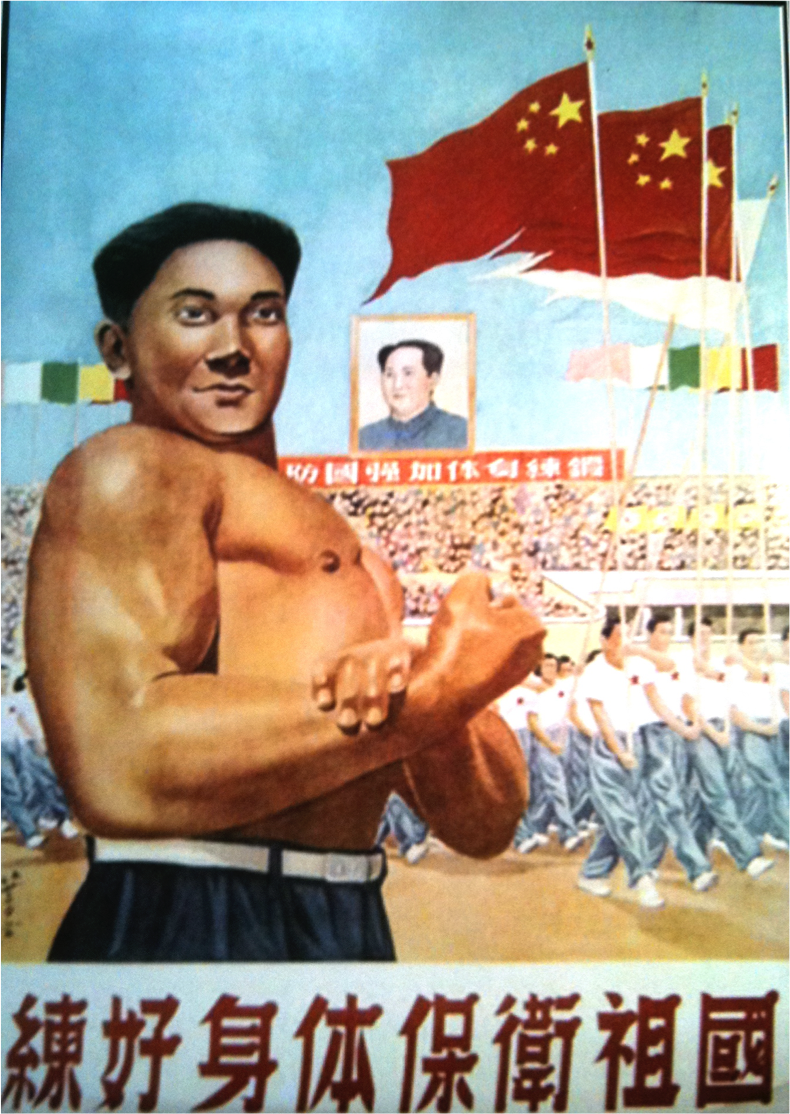
\includegraphics[width = \linewidth,scale=.7]{images/motherlandStrength.png}
      \caption{Strengthen Physique to Defend Motherland (1950)}
      \label{fig:motherlandStrength}
    \end{figure}

Along with many other facets of society after 1949, sport was institutionalised in line with Soviet bureaucratic models of governance.  In 1952 the ``State Sports (and Physical Culture) Commission'' (\textit{guojia tiyu yundon wieyuanhui} 国家体育运动委员会) (hereafter the Sports Commission) was established, which acted as the central State organ responsible for the administration of ``sport for the masses'' (\textit{qunzhong tiyu} 群众体育), ``physical culture education'' (\textit{tiyujiaoyu} 体育教育), as well as an elite competitive sport (\textit{jingji tiyu tixi} 竞技体育).  The competitive sport system was designed with the intention of creating a fast track for the development of world class athletic talent, in lieu of a sports system as advanced as other (predominantly Western) nations, whose development pathways for athletes were more organically embedded within existing social and educational institutions \citep{Brownell2008}.  By creating model athletes capable of performing and advocating the healthy, egalitarian and militaristic body promoted by the Party, competitive sport was designed to kick start more widespread engagement in ``sport for the masses'' and ``sport education''\citep[56]{Brownell1995}.

\begin{figure}[htbp]
  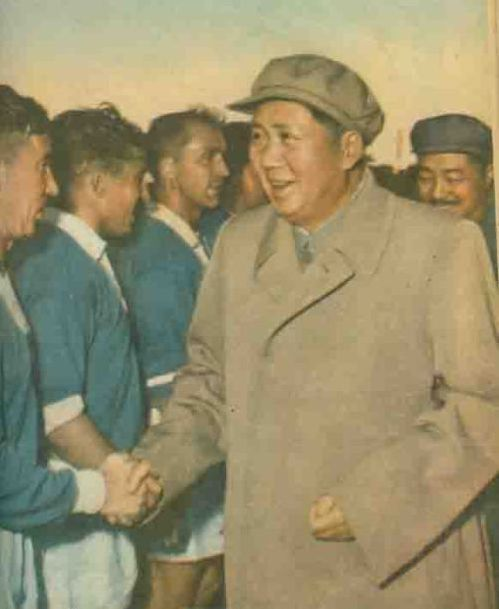
\includegraphics[scale=.5]{images/maoXNT.jpg}
  \caption{Mao Zedong congratulating members of the St Petersburg Zenit FC following a fixture against China in 1952. Source: baidu.com}
  \label{fig:maoXNT}
\end{figure}

The reinstatement of Beijing as China's capital immediately following the establishment of the People's Republic of China in 1949, had immediate implications for the Institute situated at the Temple of God of Agriculture.  The existing stadium was enlarged to a capacity of nearly 30,000, and lights were added to enable hosting training and events at night.  The stadium was host to many important sporting and political events between the years of 1949 to 1976, including a number of International football matches attended by high profile CCP members, including Mao Zedong and Zhou Enlai (see Figure ~\ref{fig:maoXNT}).

Despite becoming heavily entwined with political processes of the PRC during 1949-1976, sport and its development also became severely hampered by many factors during this period.  On the one hand, the internal political, social, and economic chaos of The Great Leap Forward (1955-58) and the Cultural Revolution (1966-77) detracted from a focus on development of sporting infrastructure and grass-roots community participation.  On the other hand, PRC's exclusion from membership in the International Olympic Committee (IOC) and thus participation in the Olympic games, limited China's ability to participate in sporting events on the International stage.






\subsubsection{Reform era tiyu (1976-2000)\label{sect:reformEra}}
The death of Mao and the end of the Cultural Revolution in 1976 signalled the beginning of widespread social and economic transformations in China, in which the development of sport was heavily implicated.  American cultural Anthropologist Susan Brownell’s work, ``Training the Body for China'' (1995) was the first and most comprehensive attempt at an anthropology of sport in China. The research that forms the basis of Brownell's monograph was conducted during the mid 1980s at a time when China was only just beginning to interact politically and economically with an international community.

In reference to the unprecedented success of the Chinese women’s volleyball team in the 1980s, including winning China's first ever gold medal in a team event at the LA Olympics in 1984, Brownell (1995: 86) explains how elite level sport functioned as a crucial symbolic practice for China in the process of ``re-joining the world.''  As a participant in the sports system as a student-athlete herself, Brownell draws on first-hand ethnographic experience of training and existing as subject to the state-administered ``microtechniques of power'' (citing \cite{Foucault1977}) designed to cultivate athletes in post-Mao China.  Brownell interrogates the role of the athlete in the perpetuation of a hyper-visible and generalisable moral order, cast in official terms as a ``socialist spiritual civilisation'' (\textit{jingshen wenming} 社会精神文明) (1995: 156).  Brownell explains that the position of the athlete in reform era China was one characterised by the tensions and shifts of an ever-transforming social terrain in China,  structured by contradictory forces of top-down state control and the emerging logic of the ``free market.''
Brownell's contribution offers the first conceptualisation of the subjectivity of Chinese athletes in the reform-era in China.

One of the most immediate transformations to effect the Chinese sports system after the death of Mao was the restoration of the High School University Entrance Examination (\textit{Gaokao} 高考, hereafter Gaokao), following the end of the Cultural Revolution in 1976 \citep[198]{Brownell1995}.  School curricula were immediately redesigned around the Gaokao, and as a result, schools quickly reduced emphases on sport programs as they were seen to draw student’s attention and energy away from academic study.  Subsequently, a situation emerged where the only option for prospective athletes was to attend a specialist sports boarding school in which a scholastic education was not emphasised or was abandoned all together in favour of intense physical training.

%Position of athletes was downgraded: derogated as a decision to sacrifice your spring (青春).

China's sporting success on an international stage in the early 1980s delayed public scrutiny of this widening gap between education and sport. The PRC won a total of 32 medals at the 1984 Los Angeles Olympics---its first official appearance at the Olympics since it boycotted the games in 1952 due to a dispute with the Republic of China (now Chinese Taipei) over the use of ``China.''  Importantly, 15 of these 32 medals were gold, and this powerful display of strength on the international stage was an enormous moment for modern Chinese nationalism in the reform era \citep{Brownell2008}.  When China produced a much less impressive performance in the summer Seoul Olympics in 1988, winning only 5 gold medals (and a total of 28), latent public criticism of way in which reform era sport had become isolated from society readily surfaced and a ``crisis in Chinese sports'' was declared \citep[199]{Brownell1995}.  Amidst broader social anxieties concerning not only the alarming quantity of the Chinese population (\textit{renkou guoduo} 人口过多), but also the problem of population \textit{quality} (\textit{renkou suzhi} 人口素质), the athlete in China was problematised as lacking sufficient ``cultural quality'' (\textit{wenhua suzhi} 文化素质) in accordance with his or her elevated social status as a ``representative'' (\textit{daibiao} 代表) of the Chinese nation on an ever-expanding international stage (General Administration of Sport 2009a; Brownell 1995: 95).

In response to this public sentiment, in 1988 former army general Wu Shaozu (伍绍祖) was appointed head of national sports commission and tasked with implementing reform measures that would help the ``societisation'' of the Chinese sport system.  In 1989 the Sports Commission adopted a policy modelled on the US college sports system, of ``combining sport and education'' (\textit{tijiao jiehe} 体教结合).  In an attempt to move away from a reliance on sport boarding schools and full-time sports training centres for the development of athletic talent, ``high level tiyu programs'' (\textit{gaoji tiyu xiangmu} 高级体育项目) were embedded within existing stand alone high schools and universities so as to ensure the ``all-round development''(\textit{quanmian fazhan} 全面发展) of the athlete \citep[203]{Brownell1995}.  As part of an emphasis on a broader range of sports and their perceived potential to facilitate community engagement, international relations, as well as commercial opportunities, various sports programs, including many non-Olympic sports such as rugby, were inducted into the Chinese sports system for the first time\citep[70]{Knuttgen1990}.

%Above all, the  democratisation of sports programs to include non-Olympic sports was driven by a persistent faith---built-in to the logic of `\textit{tiyu} form its inception in China---in the ability of sport to produce citizens of a certain \textit{quality} \citep[7]{Woronov2003}.

Reform measures in sport continued into the mid 1990s before being interrupted by China's first chance at hosting the Olympics.  In an attempt to reduce the monopolisation of power and resources in the sports system, in 1993 Wu Shaozu broke up the six major sporting bodies of the Sports Commission into 23 sports management centres, with the ultimate goal of placing every sport under the management of an independent sporting association.  In 1994, the first professional Chinese Football League was established, followed soon after by the professional Chinese Basketball League in 1995.  In 1998, the Sports Commission rebranded as the General Administration of Sport (hereafter GAS) to accord with this direction of institutional reform.  But, one year earlier in 1997, it was decided (by the powers above in the CCP) that Beijing would bid for the 2008 Olympics. As such, yet another shift in focus occurred in Chinese sport that distracted the course of reform.

By this stage in its history in China, success on the world stage at the Olympics and the increasing consumption of Chinese and international sport by China's emerging middle class meant that sport had become an important part of the Chinese national fabric \citep{Brownell}. By 2001, China had hosted the Asia Games (1990), and were preparing to bid for the Olympics.  Sport thus offered a symbolic stage on which China was able to choreograph its engagement with the world and maturation as a modern nation state.

\subsubsection{Beijing Olympics and the lost decade of sport reform (2002-2012)}

Many political and social commentators within China refer to the period under the leadership of President Hu Jintao and Premier Wen Jiabao as the ``lost decade'' (\textit{shiqu de shinian} 失去的十年) in the PRC's modern development \citep{Johnson2012}.  The main criticism by commentators is that despite China's economic rise, social and political reform during this period stagnated in comparison, leading to a deepening of problems ranging from corruption to degradation of the natural environment, to structural imbalances in Chinese economic and financial systems \citep{Barme2014,Minzner2018}.  Many commentators adopt the same stance in relation to the Chinese sport industry.

Indeed, once the bid for the Olympics was announced as successful in 2001, sport reform ground to a halt as priority shifted to winning as many gold medals as possible \citep{News2017}.  Wu Shaozu left GAS in 2000, and his two successors Yuan Weimin (袁伟民, 2000-2004) Liu Peng (刘鹏, 2004-2016) did not actively return to the project of reform, and instead continued to invest in Olympic performance.  Even though many sports had since established independent associations, these associations had to be directly affiliated with one of the 23 GAS sport management centres. Rugby, for example, became affiliated with the ``Management Centre for Small Ball Sports'' (\textit{xiaoqiu guanli zhongxin} 小球管理中心), which was also home to sports such as Golf and Ten-pin Bowling.  The structure of the sports system exists today largely unchanged, although its name changed in 1998 to ``The General Administration of Sport in China'' (\textit{Guojia tiyu zongju} 国家体育总局, hereafter GAS).

The combination of high profile scandals and corruption (match fixing, doping reports, etc.) and the persistence of China's narrow performance-focussed sports system produced palpable public discontent during the lost decade of Chinese sport.  Low investment in public team sport and deterioration of indicators of public health contributed to lack of public participation.  During this period, sports management centres swelled into sovereign entities managing large accounts. These centres thus became vulnerable to corruption and graft, and served to hinder reform despite their original design as reform facilitators.  The Chinese Basketball Association and Chinese Football Association suffered year after year of losses, and sports such as table tennis and volleyball struggled to secure a sturdy commercial foundation.  Critical murmurings remained sufficiently muffled in public discourse, however, by the strong performances of Chinese Olympic athlete delegations in Sydney 2000 (28 gold, 58 total) and Athens 2004 (32 gold, 63 total). The choreography of Chinese sporting strength on the world stage reached its pinnacle when Beijing hosted the 2008 Olympics, with the Chinese athlete delegation winning 48 gold medals in a total haul of 100 medals.  It appears that the highly visible success on the world stage distracted from much needed reforms and further institutionalised a problematic incentive structure revolving around success in Olympic sports.

%\subsubsection{the impact of competitive Olympic logic on team sports}



\subsubsection{Xi Jinping Era Sport reform and Beijing 2022 Winter Olympics (2013 - present)}

Unlike his predecessors in the post-Mao era of the PRC, when President Xi Jinping came to power at the end of 2013, he wasted no time in signalling strong intentions for immediate and major political reform as part of his tenure.  The institutional reforms initiated by Xi have had had implications for sport.  In the second half of 2014, sport was earmarked to become a ``major pillar'' of domestic economic consumption.  In 2015, the GAS released a number of policies charting a course for the transformation of the sports industry from an industry dominated by manufacturing (55\%) to a services dominated industry with a total scale of USD 800 billion by 2025 (for context, the total scale of the comparatively mature US sport industry was USD 400 billion in 2016).  In 2016, CCP Standing Committee Member, Deputy Party Secretary and former Vice Major of Beijing Gou Zhongwen was appointed Director of GAS.  Gou's appointment appeared to be a surprise move, given that Gou had no previous experience in sport. Gou is however reported to be one of Xi's trusted CCP colleagues and therefore his appointment signalled a seriousness in relation to finally executing long-awaited structural reform in Chinese sport.  Signals of this reform process include the appointment of Chinese Basketball deity Yao Ming as director of the Chinese Basketball Association (the first time a non-Bureaucrat athlete had been appointed to a top sports administration position), the removal of coaching cliques (such as the removal of Liu Guoliang as head of table tennis), and the establishment of new high performance model called ``Team China'' (\textit{beizhanban} 备战办) to kick-start elite performance ahead of the Tokyo 2020 Olympics and the Beijing Winter Olympics in 2022.  The process of reform has continued to impact on sport in China and rugby in particular.  However, these changes were largely immaterial during the period I was conducting research. The fact that a concerted effort to initiative reform was taking place around the time of my research served to highlight the problems that were the focus of reform policies.

%Late 2016:  GZW blindsided sports centre managements, calling them monopolies and saying too much power rests in the hands of their chiefs.


\section{The structure, regulations, and incentives of the Chinese Sports System}

As explained above, the Chinese Sports system has evolved gradually since it was erected at the beginning of the PRC in the 1950s. The organisational structure, and the ways in which its athletes, coaches, officials, and administrators are incentivised, however, have not changed significantly since the their inception, despite several waves of policy reform.  In this section I detail the organisational structure of the Chinese sports system, and explain the incentives that propel athletes to participate in programs such as those that exist for rugby in China.

\subsubsection{Organisational structure of the Sports System}
At the bottom of the hierarchical structure of the Sports Commission are local sports commissions (county, township and city), above which are the provincial and municipal sports commissions; and at the top is the National Sports Commission, located in Beijing \citep[59]{Brownell1995}.  The Sports Commission was responsible for all sports training centres and sports programs, of which there were many types.  On one extreme, the elite professional arm of the Sports Commission , a ``national (sport) system'' (\textit{juguo tizhi} 举国体制), which presides over all full-time professional sports teams (\textit{tigongdui} 体工队) that exist at national and provincial/municipal levels.  The main objective of this national system is to cultivate elite athletes to compete on a national and international level, in events such as the National Games (\textit{Quanguo yundonghui} 全国运动会), the Asian Games (\textit{Yazhou yundonghui} 亚洲运动会), and most importantly, the Olympic games (\textit{Aolinpike yundonghui} 奥林匹克运动会).  Due to an overwhelming Olympic-focus, all sports under the umbrella of professional arm of the Sports Commission are either Olympic sports, or Chinese martial arts (Guojia tiyu zongju 2009a).  Outside of this professional arm, elite sport programs are embedded within secondary and tertiary education institutions in a number of different ways, under the banner of the ``high school and university sport system'' (\textit{gaoxiaotizhi} 高校体制) (Guojia tiyu zongju 2009a).  At a high school level, elite sports programs are offered at ``extracurricular sports schools'' (\textit{yeyu tixiao} 业余体校), as well as regular high schools that focus on one or two sport programs in particular \citep[59]{Brownell1995}. At a tertiary level, a number of specialist sport colleges operate at national, provincial/municipal and local levels.

\subsubsection{Athlete Incentives}

Despite valorisation of the athlete as part of the proletarian revolution during the Mao era (see Section ~\ref{sect:sportPRC}), and some celebration of the nation's top athletes during the post-Mao reform era, it is clear that a career as a professional athlete is not highly desirable or coveted in China, at least not by urban elites.  It is popularly understood that becoming an athlete in China entails sacrificing one's youth (\textit{qing chun} 青春); athletes train incredibly hard and are forced to endure bitterness (\textit{chiku nailao} 吃苦奶酪).  There is a common understanding that for women in particular, the physiological demands of being an athlete (weights training, training outside, training during one's menstrual cycle) can threaten one's femininity and fertility, thus harming marriage prospects \citep{Bronwell1995}.  Although recent commercial growth of the sport industry in China has supported the rise and valorisation of ``super star'' athletes in Chinese sport, such as NBA athlete Yao Ming, or 110m hurdles Olympic Champion Liu Xiang, for most wealthy and educated urban Chinese families, the prospect of becoming an athlete does not compare to other life-course trajectories such as pursuing education.  The history of separation between the competitive sport system and the education system is also a factor in discouraging Chinese youth and their families from pursuing sport if it threatens other more attractive life course possibilities.

Nonetheless, for many sectors of society, becoming an athlete has in the past, and still does today, offer two main attractive life-course opportunities: education and employment. Entry into a competitive sport institute such as the Institute in Beijing promises access to a tertiary education and employment opportunities that tertiary level education qualifies. As I explain in more detail below, with employment also comes residency.  As such, sport offers athletes the opportunity for social mobility.  Traditionally, many athletes in China's competitive sport system are from more rural and less affluent areas.  Athletes are drawn to professional programs for the opportunity to study, find employment, and gain access to residency in urban centres and the access to education, healthcare, and other public goods that residency affords.


\myparagraph{National Athlete Technical Standards}

The Chinese competitive sport system is populated by hundreds of thousands of athletes, coaches, officials, and administrators based at hundreds of institutions throughout the country.  Professional training programs (such as the rugby program at the Institute in Beijing) exist at national, provincial, and city levels.  These programs are hosted either in standalone sport institutes, or by universities and high schools.

A series of national standards for athletes, coaches, and officials, allows for the systematic regulation of admission and performance in this system.  Standards are set out by the National governing body of each sport.  Athletes can qualify for entry to a professional sport program if they meet the nationally-defined technical standards for performance (see Figure ~\ref{}).  The lowest level of qualification for an athlete is ``Level 3'', and, as of 2010, can be achieved by recording an official level of performance in one of the following sports: Athletics, Football, Basketball, Volleyball, Table Tennis, Chinese Martial Arts, or Swimming.  Access to most ``high level sport programs'' based at universities or high schools require at least a Level 2 athlete qualification.  Admission to the Institute---a professional provincial program---necessitated a minimum Level 1 standard.  For a male athlete, a Level 1 standard could be achieved by running 11.2 seconds or faster in the 100m sprint (athletics), jumping 6m in the long jump (athletics), or achieving a top-three result in a national level tournament in football or basketball.  Once gaining entrance to the Institute, athletes were eligible to attend university if they achieved the next level of athlete qualification, that of a ``Master Sportsperson'' (\textit{yundong jianjiang} 运动健将).  This level of qualification could be achieved by representing Beijing at a national level tournament (竞体司2014).






\subsubsection{Conclusion: the logic of the Chinese Sports System}

Sport in China began as a deliberate social project driven by revolutionary goals of modernisation against the backdrop of what was perceived to be a corrupted dynastic rule.  With the establishment of the PRC, sport became a central ideological piece in China's participation with the world, which was heavily geared around participation in international multisport events such as the Olympics and the Asian Games. This explicit focus on sport as a nationalistic project has ultimately had implications for the ability of sport in China to move beyond a fixation on Olympic performance, as is demonstrated by the problematisation of the ``lost decade'' of Chinese sport and the continual challenge of developing grass-roots participation.  Despite aggressive reforms in recent years, the challenge of reform continues, and it has become clear that the founding logic of the sports system runs deep.  Thus, most athletes in China appear to be attracted to their sport by the life-course opportunities of education and future employment that participation in the professional competitive sport system offers.










  \section{The history of rugby union in China}



    \subsection{Rugby as an university level amateur sport (1992-2009)}
Although reportedly existing in China within colonial and expatriate circles for more than a century \citep[210]{Reason1979}, and as a modified military exercise as early as the 1930s \citep[135]{Morris2004}, rugby was a late entrant into the Chinese sport system, established as a ``high level sport program'' in 1990.  The advent of rugby in China was thus part of the ``democratisation'' and ``combining sport and education'' of Chinese sport initiated by Wu Shaozu during the late 1980s (see Section ~\ref{sect:reformEra}).   The introduction of rugby into China was initiated originally at CAU by professor Shi Zhengsheng (施振声) who was introduced to rugby by his
supervising professor while completing vocational studies at Azabu University in Japan 1987-1989 \citep{Xu2010}.  Following Shi’s return to CAU, an exchange relationship was set up between the two universities, and throughout 1990, coaches and referees from Azabu University came to CAU to help set up the necessary infrastructure required for a rugby program.  On the 12th December 1990, China’s first rugby union team was created.  The program was originally made up of existing CAU students who expressed interest in the novel activity, but by its second year, the program earned status as a High Level Sport Program and was subsequently advertised to student-athletes across the country \citep[2]{Xu2010}.  Between 1990 and 2009, rugby programs based on this original CAU model were established within over 30 regular universities and specialist sports colleges in cities throughout China.  There are also a number of social rugby clubs (\textit{shehui julebu} 社会俱乐部), organisations completely independent of the state sports system, in major cities with high expat populations (e.g., Shanghai, Beijing, Chengdu, Qingdao).

The Chinese Rugby Football Association (CRFA) was established in 1997. Both the men and women’s national teams, made up of players predominantly from CAU, but also from other well-established programs based at the Shanghai Sports University, Shenyang Sports College, and the People’s Liberation Army Sports College. China consistently competes against other nations in the Asia Pacific region (most notably in the Asian Games and the East Asian Games), and is also occasionally involved in top-tier international tournaments such as the International Hong Kong Sevens.

For the first 20 years of its existence in China, Rugby was part of a large collection of ``cold-gate'' sports (\textit{lengmen xiangmu}, a term that refers to a profession, trade or branch of learning that receives little attention) in China, which had a relatively small participation base compared to other interactive team sports like basketball or football.  While football and basketball have matured as standalone enterprises with supporting market-based consumer industries, most other sports in China (i.e., all other Olympic events, including rugby) exist primarily due to the support of the enormous state-sponsored sport system.  Whereas the commercial basketball and football industries might offer a small percentage of prospective athletes incentives of fame and fortune, the benefits of a state-sponsored sports programs like rugby are more modest.  Chinese youth either gravitate or are ushered by their parents towards sporting careers primarily due to potential life-course opportunities such as access to tertiary education and post-athletic career employment.


\subsection{Rugby in China 2010 - 2013 \label{sect:rugbyinChina}}
Olympic status transformed rugby almost overnight from its former position as an amateur sport played at university level by a handful of universities.  In 2010, rugby (in its seven-a-side version of rugby sevens) was included as one of 33 events to be held at the 2013 National Games in the city of Shenyang. This decision spurred provinces to set up professional rugby programs at provincial sports institutes, to compete at the National Games in 2013.  Ten of China's collection of 32 provinces and municipalities that participate in the National Games have full time men's and women's rugby programs.  The most important measure success in sport is derived from results in the National Games (\textit{quanguo yundonghui} 全国运动会) \citep{Hong2002}.  The amount of funding a province and its provincial sporting institutes and programs receive is decided to a large extent by results at the national games.

When rugby union was officially inducted into the state sponsored sports system in 2010, a total of five full time Men's (Beijing, Shandong, People's Liberation Army (PLA), Liaoning, and Shanghai) and six Women's (Beijing, Shandong, Anhui, Liaoning, Shanghai, and Jiangsu) provincial programs were established, signalling a intention to invest in the sport for the long term.  With professional provincial rugby programs catering for tertiary aged athletes (17 years and above) already established, these provinces could also initiate the establishment of city level rugby programs catering for high school aged athletes (10 - 16 years).  In this way, a previously non-existent development pathway for athletes, coaches, and officials began to emerge in provinces interested in investing in the sport.

% a quadrennial multi-sport event hosted on rotation by provincial capital cities
 Full time programs could draw fully on the institutional resources of their respective provinces to offer athletes a range of attractive life-course opportunities relating to education, employment, and permanent residency.  In the case of the Men's and Women's programs based at the Institute, for example, athletes were attracted by the offer of much sought after Beijing permanent residency, the opportunity to attend a well-renowned Beijing university, and the chance to remain at the Institute as an employee after their career as an athlete.  All of these opportunities were of course conditional on various hurdles of measurable performance.  Resources of provincial sport institutes also included athletes from adjacent programs such as athletics or association football.  Full time rugby programs soon began to attract transition athletes from these sports, which were often overcrowded due to their traditional popularity.

In addition to these full time provincial programs, three part-time men's (Inner Mongolia, Heilongjiang, and Xinjiang) and two part-time women's (Sichuan and Xingjiang) programs were established, in which these provinces temporarily employed rugby athletes from university programs. In addition, Hong Kong fielded both a Men's and a Women's side, bringing the total of Men's and Women's teams eligible to compete in the National Games to nine and ten, respectively.


\subsubsection{The National Games 2013 \label{sect:fallFromGrace}}
A few provinces in particular identified an opportunity to achieve a beneficial result at the National Games by heavily investing in this debutant sport.  The Beijing men's and women's programs (based at the Institute) managed to attract a large amount of China's existing rugby talent from where it was previously based at the CAU, Beijing.  Importantly, among Beijing's recruits was the unofficially touted ``Boss''  (\textit{Laoda} 老大) of Chinese rugby, Chinese national coach Zheng Hongjun.  Meanwhile, Shandong province, a powerhouse in other provincial sports, succeeded in attracting the majority of the remaining rugby talent.  The pull to Shandong was strong for a large majority of rugby players in China at the time, many of which were originally from Shandong.\footnote{(Indeed, a large proportion of athletes more generally are from Shandong, \citep[see][]{Taylor2010}.}  Importantly, the talent transferred to Shandong province also included coaching staff, namely Zheng Hongjun's student and soon to be rival, former Chinese Women's Team coach, Lu Xiaohui.  Besides Beijing and Shandong, Jiangsu and Anhui province were strong contenders for the Women's gold medal, while the People's Liberation Army (PLA) and Hong Kong in particular were strong contenders for top spot in the men's competition.

Beijing's results in the two years leading into the 2013 national games were strongest overall across the men's and women's teams.   However, the traditionally strong Hong Kong men's and women's teams had only occasionally participated in these tournaments due to conflicting international tournaments.  In the semi-finals of the National Games, held in Shenyang at the beginning of September 2013, the Beijing men came up against Hong Kong, while the Shandong men played off against the PLA.  Beijing lost to their stronger and more favoured opponents, and Shandong beat the PLA.  Meanwhile in the women's tournament, both Beijing and Shandong advanced to the final without faltering.  The stage was set: the traditional favourites, Beijing, led by the reining Boss of Chinese rugby, would face Shandong---the underdogs---lead by the Boss's cunning apprentice come challenger.

The men's final was played first, and in somewhat of an upset, Shandong edged out Hong Kong to win the gold medal by one try (one five-point touch down).  In the women's final, scores were level until early in the 2nd half when Shandong went ahead by two tries to nil.  At that point, the Beijing women's team, under instruction from their coach Zheng Hongjun, suddenly stopped playing.  After being asked by the referee and match officials to continue, the Beijing athletes stood firm and refused to play on, forming a huddle on their side of half-way in the middle of the field. Shandong had no choice but to continue to play out the rest of the 2nd half, running in try after try, until the final score at full time was a farcical 71-0 \citep{Sina2013}.  Shandong was declared victorious, while Beijing called foul play, claiming that the Spanish referee had been unfairly adjudicating the match in Shandong's favour.  The details and dramas of this now well-known story in China's sporting history (known as ``The 2013 National Games Match Strike Scandal'' (13年全运会巴塞门) ) require more detailed development in a format that exists beyond the scope of this particular dissertation.  Suffice to say, the repercussions of this incident for the Beijing provincial rugby program were extremely costly.

\subsection{Temple of the God of Agriculture Sports Institute}
The rugby match-striking-gate of 2013 led to a sudden fall from grace for the Beijing rugby programs.  Between 2010 and 2013, the Institute Leadership, excited about the prospect of unprecedented success at the national games,  immediately elevated the rugby programs to top-priority status.  Rugby received unrivalled institutional and financial support in the hope that both teams would be crowned National champions---what would have been the Institute's first National Games gold medals since 2004.  During this period, the rugby program attracted a high profile sponsorship deal from Beijing Capital Steel (北京首钢), which enabled the Institute to invest in a team of foreign coaches from New Zealand to come to Beijing on a periodic basis to consult on training and preparation. Both teams also travelled twice to New Zealand for two three-month stints of off-season training and competitions.  Between 2010-2013, the rugby team lived in the Institute's best available accommodation, and ate their meals at the Institute's highest level canteen, reserved for National-level champions.  Right up until the National Games in 2013, the men's and women's teams had met the high expectations placed on them, winning all but one of seven national tournaments each.  All indications were positive for Beijing to take home two gold medals.  However, as explained above, the National Games in Shenyang in September 2013 did not transpire as Beijing would have hoped.

In the end, Beijing came away with one bronze medal (men's team) and one face-destroying disqualification for the women.  The assistant coach of the Beijing men's team, Shi Yan, told me quietly one evening that the Beijing women's rugby team was the first Beijing team in the 48-year history of the National Games not to receive the ``medal for civilised spirit''  (awarded by the Beijing Mayor to all Beijing representatives in the National Games) (SOURCE).  All rugby coaches and many senior athletes of the 2013 National Games campaign have since left the Temple of Agriculture, either retiring or moving to other provinces.  The rugby program was all but abandoned at the end of 2013, with athletes from both teams being told to take a break for an undetermined length of time.  It wasn't until April 2014 that the men's program was resurrected with the appointment of a new head coach.  It was in this context that I entered the Institute and began ethnographic research.



\section{Qualifications and position of the researcher}

One question yet to be answered is: how do know so much about rugby in China?

Before arriving in Beijing in 2015 to begin my doctoral research, the last time I was in China was two years earlier in 2013, when I spent eight months coaching the Chinese men's youth rugby 7s team in the lead up to the Nanjing Asian Youth Olympics.  Before that, I had spent one year studying on Exchange at Beijing University in 2008, and another year before that on an intensive Chinese language course at Liaoning University, Shenyang, in 2006---my first trip to China.  Rugby featured heavily in both instances.  In 2006, an Australian classmate and friend Ed had caught wind of the fact that there was a rugby program down the road from Liaoning University at the Shenyang Sports College (SSC).  Despite the fact that we had both been diligently attending class and courageously deploying our elementary Chinese to order food at restaurants and befriend local taxi drivers, Ed and I were, nonetheless, three months into our intensive language exchange and feeling that our Chinese skills were floundering.  We suspected that this was in large part due to the fact that we had met very few local Chinese people our age.  So one afternoon we rode our bikes over to the Shenyang Sports College in time for the rugby team's afternoon training session.  Less than six months later, we were boarding an overnight train from Shenyang to Shanghai with the SSC rugby team to compete in the annual Shanghai Rugby 7s Tournament.  We had become closely integrated into the community of rugby athletes at SSC, due in part to the common language of rugby that we all shared, and perhaps mostly due to the overwhelming hospitality of the SSC athletes and coaches.  The decision to find the rugby team may have also helped us improve our Chinese. Ed and I were the only two in our cohort to finish the year in Shenyang with a Level 6 in the Chinese Proficiency Exam, which qualified us to study alongside Chinese local students at an undergraduate level.

    Buoyed by this experience with the SSC rugby team in 2006, I followed a similar template two years later when I arrived at Beijing University on exchange from Sydney University to study sociology at Beijing University.  I had just finished working at the 2008 Beijing Olympics. At that time in Beijing, the only Chinese rugby program was based at the Chinese Agricultural University, a forty minute cycle north of Beijing University.  It was during my time training and generally ``hanging out'' at CAU that I met and developed a strong friendship with Kai, who was at the time playing for CAU and China, while also finishing a Master's degree in Labour Law.  I also met and developed relationships with many rugby players, coaches, and general fans of the Beijing rugby community.  The CAU rugby program was the strongest in the country: CAU consistently outperformed its rivals at the time (Shanghai Sports Institute, the People's Liberation Army, and SSC) and it was awarded with the responsibility of hosting the Chinese national team.  When the International Olympic Committee announced in late 2009 that rugby would be played in the 2016 Rio De Janeiro Olympics, it was subsequently decided in 2010 that rugby would be inducted into the state sponsored sports system and played in the next Chinese National Games in 2013.  Following this announcement, many of CAU's athletes and coaches dispersed to various professional provincial rugby programs, the main ones being Beijing and Shandong.

    Between 2009 and 2013 I returned to Australia to finish my undergraduate degree, during which time my own rugby career also rapidly developed.  After a successful season in the Sydney Premiership competition in 2009, I was selected to play for the Australian Rugby Sevens Team. I represented Australia from 2009 through to the end of 2012.  In 2013, during the 9 month gap between my Australian rugby contract ending and the start of my graduate studies at Oxford University, I returned to China to coach the Chinese Youth Men's 7s program in their lead-up to the 2013 Nanjing Asian Youth Olympics.  Along with a small team of Chinese coaches and management, I coached a core group of roughly 25 athletes aged between 15 and 18 years old. We trained 6 days a week for approximately 6 months, with only occasional breaks for National holidays, or for athletes to return to their home provinces to complete compulsory exams.  The program was based predominantly in Anhui province, and we travelled from Anhui to other provinces further afield to find suitable practice opportunities against provincial programs.  Soon after the completion of the Asian Youth Olympics in Nanjing in 2013, the Chinese National Games were held in Shenyang. Rugby was played---for the first time in National Games history---with dramatic consequences, explained above.




\section{Conclusion}

                                                          \end{CJK}
